\chapter[Improved Bipartition Cover Bound]{An Improved Bipartition Cover Bound for the Multispecies Coalescent Model}
\setcounter{secnumdepth}{2}

% Background
\section{Introduction}
\label{sec:introduction}

Consensus methods have grown in popularity in phylogenetics as
large genomic datasets have revealed the limits of single-gene
tree inference. Evolutionary processes such as incomplete lineage
 sorting, gene duplication and loss, and horizontal gene transfer
 can cause individual gene trees to differ from the true species
 tree. Consensus and summary-based methods aim to reconcile this
  discordance by aggregating information across many loci,
  providing statistically consistent estimates of species
  relationships under realistic models of gene tree variation.

However, even for a relatively small number of species, the space of possible species tree
topologies is intractably large. Because of this, it is often necessary to reduce the
search space somehow. One common strategy uses the \emph{bipartitions} of the underlying phylogenetic tree $\cT^*$.
Each edge $e$ of $\cT^*$ induces a bipartition of its leaf set $\cL$: deleting $e$ produces two connected components,
whose leaf sets form the two parts of the bipartition. By Buneman's splits-equivalence
theorem (see, e.g., \cite[Theorem~3.1.4]{semple2003_phylogenetics}), these bipartitions uniquely
characterize $\cT^*$. It is therefore natural to restrict the search to species trees whose
bipartitions belong to a candidate set obtained from the input gene trees, possibly extended
using additional heuristics. This strategy is employed by several modern phylogenetic
methods, including FastRFS
\cite{vachaspati2017_fastrfs_robinson_foulds_supertrees} and the widely used ASTRAL
family: ASTRAL \cite{mirarab2014_astral_species_tree_estimation}, ASTRAL-II
\cite{mirarab2015_astral_ii_species_tree_estimation}, ASTRAL-III
\cite{zhang2018_astral_iii_species_tree_reconstruction}, and wASTRAL
\cite{zhang2022_weighting_gene_tree_uncertainty}.

    In the case the true species tree lies in this restricted space, we say the gene trees form
    a \textit{bipartition cover} of the species tree. When this occurs, ASTRAL comes with some strong
    finite-sample guarantees \cite{shekhar2018_how_many_genes_are_enough}. When it does not occur,
    ASTRAL provides no guarantees on how the estimated tree will relate to the true species tree. As a result,
    it is important to understand the likelihood of such a cover when assessing whether these finite-sample guarantees apply.
    Moreover, since an experimenter must decide how many loci to collect before the underlying species
    tree topology is known, they cannot calibrate the required sample size to that topology. A topology-free upper bound
    provides a conservative benchmark for the sample size required to obtain a bipartition cover with a prescribed
    probability. Under the \emph{multispecies coalescent model (MSC)}, the paper by \citet{uricchio2016_bipartition_cover} develops
    such a bound as a function only of two key parameters: the number of species $k$ and the minimum
    branch length $T_{\mathrm{min}}$ of the tree.

    In this chapter, we identify a few areas where this existing bound
    is lossy and develop some topology-free improvements. Our main contributions come from careful analysis
    of various ``worst cases'' of the MSC model: species tree topologies that somehow make coalescence
    difficult and certain bipartitions challenging to recover. Beyond this, since all these bounds are
    complicated functions of the underlying parameters, we develop some asymptotics to describe
    the growth rates of these bounds as functions of these parameters in a few natural regimes.

Throughout, suppose we have a species tree $\cT^*$ with $k$ species and minimum branch
length $T_{\mathrm{min}}$. For $q\in(0,1)$, define
\[
N_{\mathrm{cov}}(q;\cT^*)
:=\inf\{n\in\N:\P(G_1,\ldots,G_n\text{ form a bipartition cover of }\cT^*)\geq q\},
\]
where the $G_i$ are independent gene trees generated from $\cT^*$ under
the MSC model, as described below. Namely, $N_{\mathrm{cov}}(q;\cT^*)$ represents the minimal number of
independent gene trees required to recover the underlying species tree $\cT^*$ with the
prescribed probability $q$. In this chapter, our goal is to upper bound this quantity.


\subsection{The Multispecies Coalescent Model}
\label{sec:multispecies-coalescent-model}

We start with a brief discussion of the \textit{multispecies coalescent (MSC) model},
the probabilistic model underlying all the theoretical guarantees of ASTRAL and many other phylogenetic
 inference algorithms. The MSC model describes how gene tree topologies are generated from a
 given species tree \citep{yang2003_bayes_species_divergence_ancestral_population,rannala2020_multispecies_coalescent_species_tree_inference}. It is in a sense the simplest model
 that can explain the phenomenon of \textit{incomplete lineage sorting (ILS)}, the observation
 that the most common gene tree topology can differ from the species tree topology.
 This phenomenon makes species tree inference difficult: the intuitive ``majority vote'' estimator
  is not consistent.

The MSC model is essentially just a constrained version of Kingman's coalescent: going backwards in
time along each branch of the species tree, we assume the surviving gene lineages coalesce according
to Kingman's coalescent. Namely, each pair of lineages coalesce at rate one. Figure~\ref{fig:msc_model}
gives an example of the MSC model and illustrates how gene tree topologies can differ from the species tree.
More concretely, let

\begin{equation}
    g_{ij}(T) := \sum_{k=j}^i \frac{\exp(-\binom{k}{2}T) (2k-1)(-1)^{k-j}j_{(k-1)} i_{[k]}}{j!(k-j)!i_{(k)}}
    \label{eqn:def_of_g_ij}
\end{equation}

\noindent be the probability that $i$ lineages coalesce into exactly $j$ lineages in
 time $T$ under Kingman's coalescent. Here $a_{(k)} = a(a+1) \cdot ... \cdot (a+k-1)$ and $a_{[k]} = a(a-1)\cdot ... \cdot (a-k+1)$
 denote the rising and falling factorial respectively, and the time $T$ is measured in coalescent units. The function $g_{ij}(T)$
 is the basis of the original bound in \citet{uricchio2016_bipartition_cover} and
  all the new bounds we develop. In the setting of the MSC model, $T$ represents
   the length of a given branch of the species tree, and $g_{ij}(T)$ describes the
   distribution of the number of lineages that remain uncoalesced at the end
   of that branch if we start with $i$ lineages.



\begin{figure}
    \centering
    
\includegraphics[width=0.5\linewidth]{msc_model.PNG}
    \caption{Two different gene trees generated from the same species tree under the multispecies coalescent model. The black lines outline the underlying species tree topology, and the colored lines indicate the gene lineages}
    \label{fig:msc_model}
\end{figure}


% Original Bound
\subsection{The Original Bound and Main Contributions}
\label{sec:original-bound-main-results}

Under the MSC model, \cite{uricchio2016_bipartition_cover} establishes the following bound.

\begin{theorem}[Original Bipartition Cover upper bound]
\label{thm:uricchios_bipartition_cover_bound}
%
\begin{equation}
     M_o(k,T_{\mathrm{min}}) := \frac{\log\left(\frac{1-q}{k-3}\right)}{\log \left(1-g_{k-2, 1}(T_{\mathrm{min}})\right)}
     \label{eqn:uricchios_bipartition_cover_bound}
\end{equation}
%
\noindent satisfies $N_{\mathrm{cov}}(q;\cT^*)\leq \lceil M_o(k,T_{\mathrm{min}})\rceil$.
\end{theorem}


\noindent In this work, we aim to develop a topology-free improvement of this upper bound.
Our work relies on careful analysis of various ``worst-case'' topologies when it comes to phylogenetic inference. For this purpose, we define two tree types: a \textit{caterpillar tree} and a \textit{balanced tree}.

A \textit{balanced tree} is any rooted tree so that for every vertex the number of leaves in its two subtrees differs by at most one. A \textit{caterpillar tree} is a tree where every non-leaf vertex has one child who is a leaf. Figure \ref{fig:caterpillar_and_balanced_tree} provides a simple illustration.

% fig
\begin{figure}[h!]
\centering
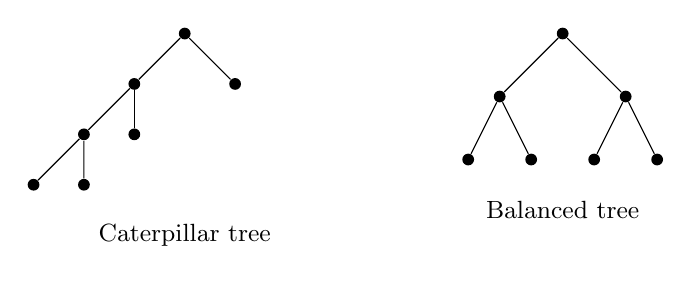
\begin{tikzpicture}[scale=0.8]

% Caterpillar
\begin{scope}[xshift=-3cm]
\node[circle, fill=black, inner sep=1.5pt] (root) at (0,0) {};
\node[circle, fill=black, inner sep=1.5pt] (n1) at (-0.8,-0.8) {};
\node[circle, fill=black, inner sep=1.5pt] (n2) at (0.8,-0.8) {};
\node[circle, fill=black, inner sep=1.5pt] (n3) at (-1.6,-1.6) {};
\node[circle, fill=black, inner sep=1.5pt] (n4) at (-0.8,-1.6) {};
\node[circle, fill=black, inner sep=1.5pt] (n5) at (-2.4,-2.4) {};
\node[circle, fill=black, inner sep=1.5pt] (n6) at (-1.6,-2.4) {};

\draw (root) -- (n1);
\draw (root) -- (n2);
\draw (n1) -- (n3) ;
\draw (n1) -- (n4);
\draw (n3) -- (n5);
\draw (n3) -- (n6);

\node at (0,-3.2) {\small Caterpillar tree};
\end{scope}

% Balanced
\begin{scope}[xshift=3cm]
\node[circle, fill=black, inner sep=1.5pt] (root) at (0,0) {};
\node[circle, fill=black, inner sep=1.5pt] (n1) at (-1,-1) {};
\node[circle, fill=black, inner sep=1.5pt] (n2) at (1,-1) {};
\node[circle, fill=black, inner sep=1.5pt] (n3) at (-1.5,-2) {};
\node[circle, fill=black, inner sep=1.5pt] (n4) at (-0.5,-2) {};
\node[circle, fill=black, inner sep=1.5pt] (n5) at (0.5,-2) {};
\node[circle, fill=black, inner sep=1.5pt] (n6) at (1.5,-2) {};

\draw (root) -- (n1) ;
\draw (root) -- (n2);
\draw (n1) -- (n3);
\draw (n1) -- (n4);
\draw (n2) -- (n5);
\draw (n2) -- (n6);

\node at (0,-2.8) {\small Balanced tree};
\end{scope}
\end{tikzpicture}

\caption{The two main extremal tree topologies: caterpillar and balanced trees}

\label{fig:caterpillar_and_balanced_tree}
\end{figure}
% end fig

% deleted fig


These two tree topologies represent opposite extremes for coalescent behavior: one maximally balanced and the other maximally unbalanced. Caterpillar trees present a combinatorial bottleneck for phylogenetic inference, as many of their bipartitions involve very large subsets of taxa. Balanced trees, however, present a more subtle and severe difficulty: they induce a \emph{coalescent bottleneck}, in which lineages are so evenly dispersed that coalescence is systematically delayed.

This distinction is made precise in Lemma~\ref{lem:caterpillar_maximize_increasing_sums}, which identifies caterpillar trees as extremal for increasing functions of descendant counts, and in Lemma~\ref{lem:balanced_is_worse_case}, which shows that balanced trees are stochastically worst-case for the number of surviving lineages under the multispecies coalescent. Together, these lemmas underpin our main result, which appears as Theorem~\ref{thm:improved_bipartition_cover_bound_balanced} below.

\begin{theorem*}
For $\ell\geq 2$, let $w_\ell(T)$ denote the probability that the lineages descending
from a balanced $\ell$-taxon tree, with all branch lengths equal to $T$, coalesce to a single
lineage. Then
\[
N_{\mathrm{cov}}(q;\cT^*)\leq
\inf\left\{n\in\N:
    \sum_{\ell=2}^{k-2}\bigl(1-w_\ell(T_{\min})\bigr)^n\leq 1-q
\right\}.
\]
In particular,
\[
N_{\mathrm{cov}}(q;\cT^*)\leq \left\lceil
    \frac{\log\!\left(\frac{k-3}{1-q}\right)}
         {-\log\!\left(1-w_{k-2}(T_{\min})\right)}
\right\rceil.
\]
\end{theorem*}

\noindent Due to the recursive structure of a balanced tree, these probabilities $w_\ell$ are easy
to compute. Empirically, we observe this improves over Theorem \ref{thm:uricchios_bipartition_cover_bound} by
several orders of magnitude in some regimes, especially when the minimum branch length $T_{\mathrm{min}}$ is small.

Analytically, we show in this short-branch regime this new bound improves upon the original
by a factor exponential in the inverse minimum branch length; Lemma~\ref{lem:improvement_ratio_asymptotics} makes
this precise.

For clarity of exposition, we postpone several short technical results and their proofs to the appendix.


%%%%%%%%%%%%%%%%%%%%%%%%%%%%%%%%%%%%%%%%%%%%%%%%%%%%%%%%%%%%%%%%%%%%%%%%%%%%%%%%%
% Topology-free improvements
%%%%%%%%%%%%%%%%%%%%%%%%%%%%%%%%%%%%%%%%%%%%%%%%%%%%%%%%%%%%%%%%%%%%%%%%%%%%%%%%%
\section{Topology-Free Improvements to the Original Bound}
\label{sec:topology-free-improvements}

\subsection{Sources of Loss in the Original Bound}
\label{sec:sources-of-loss}

To guide our work, we outline the proof of the original bound, and identify where it is lossy.

\begin{proof}[Proof Outline of Theorem \ref{thm:uricchios_bipartition_cover_bound}]
Every tree contains the \emph{trivial bipartitions} $\{x\} | (\cL - \{x\})$, so we may
restrict attention to nontrivial bipartitions. There are $k-3$ \emph{nontrivial bipartitions} in a
species tree: one for each internal edge\footnote{There are $k-2$ internal edges, but the two
edges adjacent to the root induce the same, possibly trivial, bipartition.}.
\begin{enumerate}
    \item By union bound we can just bound the probability a specific species tree bipartition occurs in the gene trees.

    \item  By independence of gene trees we can reduce to the case of a single gene tree.

    \item Suppose $\phi_e$ is the bipartition associated to edge $e$ in a species tree. One way $\phi_e$ can occur in the gene tree is if all lineages below $e$ coalesce by the time they exit $e$. If there are $\alpha_e$ such lineages, we can lower bound this probability by the probability $\alpha_e$ lineages coalesce down to one along just the single edge $e$.

    \item The worst-case for the previous step is if edge $e$  is as short as possible (length $T_{\mathrm{min}})$ and the number of lineages that have to coalesce is as large as possible $(\alpha_e = k-2$ since $\phi_e$ is nontrivial).
\end{enumerate}

If we let $E_n$ be the event all bipartitions occur in $n$ gene trees and $E_{i,n}$ be the event bipartition $\phi_i$ occurs in at least one of the $n$ gene trees, then combining the above gives
%
\begin{align*}
    \P(E_n) & \geq 1 - \sum_{i=1}^{k-3} (1-\P(E_{i,n}))\\
    %
    &  \geq 1 - (k-3)  \cdot \max_i (1-\P(E_{i,n})) \\
    %
    & = 1 - (k-3) (1- \min_i \P(E_{i,1}))^n \\
    %
    & \geq  1 - (k-3) (1- g_{k-2, 1}(T_{\mathrm{min}}))^n
\end{align*}
%
\noindent from which we can invert to find the bound on $n$.
\end{proof}


% Improvement 1
\subsection{Descendant Counts and Caterpillar Extremality}
\label{sec:first-improvement-descendant-counts}

For an edge $e$, let $\alpha_e$ denote the number of leaves below $e$, namely leaves in the
connected component of $\cT^* \setminus \{e\}$ not containing the root. When an edge $e_i$ is
indexed, we define $\alpha_i := \alpha_{e_i}$. We call the set
%
    \[\{\alpha_i\}_{i=1}^{k-3} := \{\alpha_e : \text{e generates a nontrivial bipartition}\}\]
%
\noindent the \emph{descendant counts} of $\cT^*$. Since both edges adjacent to the root generate
the same bipartition, there is some ambiguity in how we define the descendant counts. To resolve this,
we always choose the edge adjacent to the root with fewer descendants, although this choice is inconsequential.
An example is given in Figure \ref{fig:example_descendants_alpha_i}.

One step at which the proof of Theorem \ref{thm:uricchios_bipartition_cover_bound} is lossy is that we essentially bound

\[\P(E_{i,1}) \geq g_{\alpha_{i}, 1}(T_{e_i}) \geq g_{k-2, 1}(T_{\mathrm{min}}),\]

% Example alpha_i
\begin{figure}[h]
\centering
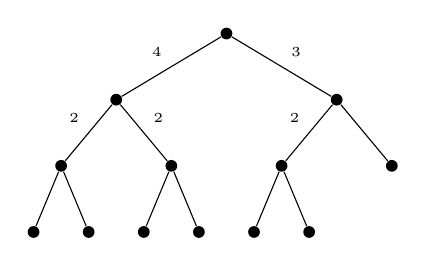
\begin{tikzpicture}[scale=0.7]

\node[circle, fill=black, inner sep=1.5pt] (root) at (0,0) {};
\node[circle, fill=black, inner sep=1.5pt] (n1) at (-2,-1.2) {};
\node[circle, fill=black, inner sep=1.5pt] (n2) at (2,-1.2) {};
\node[circle, fill=black, inner sep=1.5pt] (n3) at (-3,-2.4) {};
\node[circle, fill=black, inner sep=1.5pt] (n4) at (-1,-2.4) {};
\node[circle, fill=black, inner sep=1.5pt] (n5) at (1,-2.4) {};
\node[circle, fill=black, inner sep=1.5pt] (n6) at (3,-2.4) {};
\node[circle, fill=black, inner sep=1.5pt] (n7) at (-3.5,-3.6) {};
\node[circle, fill=black, inner sep=1.5pt] (n8) at (-2.5,-3.6) {};
\node[circle, fill=black, inner sep=1.5pt] (n9) at (-1.5,-3.6) {};
\node[circle, fill=black, inner sep=1.5pt] (n10) at (-0.5,-3.6) {};
\node[circle, fill=black, inner sep=1.5pt] (n11) at (0.5,-3.6) {};
\node[circle, fill=black, inner sep=1.5pt] (n12) at (1.5,-3.6) {};

\draw (root) -- (n1) node[midway, above left] {\tiny 4};
\draw (root) -- (n2) node[midway, above right] {\tiny 3};
\draw (n1) -- (n3) node[midway, above left] {\tiny 2};
\draw (n1) -- (n4) node[midway, above right] {\tiny 2};
\draw (n2) -- (n5) node[midway, above left] {\tiny 2};
\draw (n2) -- (n6);
\draw (n3) -- (n7);
\draw (n3) -- (n8);
\draw (n4) -- (n9);
\draw (n4) -- (n10);
\draw (n5) -- (n11);
\draw (n5) -- (n12);
\end{tikzpicture}
\caption{Example of the descendant counts $\{\alpha_i\}$ associated to the nontrivial bipartitions/edges of a phylogenetic tree. Note there is some subjectivity in deciding which edge adjacent to the root to take: depending on our choice our descendant counts would either be $\{\alpha_i\} = \{4,2,2,2\}$ or $\{\alpha_i\} = \{3,2,2,2\}$. To remove ambiguity, we always choose the edge with the least descendants.}
\label{fig:example_descendants_alpha_i}
\end{figure}
% end fig


For most edges $e$, the number of descendants $\alpha_{e}$ is far smaller than the total number of species $k$.
By Lemma \ref{lem:cdf_of_Zi}, we know $\ell \mapsto g_{\ell 1}(T_{\mathrm{min}})$ is a
decreasing function of $\ell$: the more lineages we start with, the harder it is to coalesce down to one.
As a result, this second approximation $g_{\alpha_{i}, 1} \geq g_{k-2, 1}$ can be quite lossy. Nonetheless, to derive
a topology-free bound we must assume these $\alpha_i$ are in a sense as large
as possible. The following makes this precise.

\begin{lemma}[Caterpillars Maximize Increasing Sums]
\label{lem:caterpillar_maximize_increasing_sums}
Suppose $\{\alpha_{i}\}_{i=1}^{k-3}$ are the descendant counts of our rooted binary tree $T$. Moreover, suppose $f: \N \to \R$ is nondecreasing. Then $\sum_i f(\alpha_{i})$ is maximized when $T$ is the caterpillar tree, in which case $\{\alpha_{i}\} = \{2,3,..., k-2\}$.

\end{lemma}

\noindent The result is true regardless of our convention for choosing the edge adjacent to the root.
Moreover, it is clearly also true if we use \textit{all} descendant counts
$\{\alpha_i\}_{i=1}^{2k-2}$ rather than just those corresponding to nontrivial bipartitions:
all but one of the additional $\alpha_i$ are equal to one, and it is clear from the proof below
that we can handle the exceptional value as well.

\begin{proof}[Proof of Lemma \ref{lem:caterpillar_maximize_increasing_sums}]
    Since $f$ is nondecreasing, it suffices to show we can reindex $\{\alpha_i\}_{i=1}^{k-3}$ so
    $\alpha_i \leq i + 1$. Heuristically, we are just pairing up each edge $e$ in our
    tree $T$ with an edge $e'$ in our caterpillar tree so that $e$ has at most as many descendants as $e'$.
    We induct on $k$.

    % Base case
    If $k=4$, the two unique rooted trees, shown in Figure~\ref{fig:caterpillar_and_balanced_tree},
    both have $\alpha_1 = 2$ for their only nontrivial bipartition, so the
    statement is trivially true.

    Otherwise, suppose we have a tree $\cT$ with $k > 4$ leaves. Suppose the two subtrees of the root contain
    $m,r$ leaves respectively. There are two cases:

    \begin{enumerate}[label=(\alph*)]
        \item \textit{Either $m \leq 2$ or $r \leq 2$}. If $\cT'$ is the larger subtree of the root, by induction we can reindex
        its descendant counts $\{\alpha_i\}_{i=1}^{k-4}$ so $\alpha_i \leq i+1$. The edge $e$ connecting $\cT'$ to the root
        trivially has $\alpha_e \leq k-2$, as all nontrivial bipartitions in $\cT$ do, we can pair this remaining edge $e$ with
        the top nontrivial edge of our caterpillar tree.

        \item \textit{Both $m, r \geq 3$}. Let $\cT', \cT''$ be the two subtrees of
               the root with $m,r$ leaves respectively, and
               let $\{\kappa_i\}_{i=1}^{r-3}$ and $\{\beta_j\}_{j=1}^{m-3}$ be their descendant
               counts. If $r<4$ (respectively, $m<4$), the corresponding subtree has no nontrivial
               bipartitions, and we take the family $\{\kappa_i\}$ (respectively, $\{\beta_j\}$) to be empty.
               By induction, these can be ordered so $\kappa_i \leq i+1$ and $\beta_j \leq j+1$.
               Clearly then defining

        \[\alpha_i = \begin{cases}
            \kappa_i, & 1 \leq i \leq r-3, \\
            \beta_{i-r+3}, & r-3 < i  \leq k-6. \\
        \end{cases}\]

        \noindent Namely, we list the edges of $\cT'$ first, and then the edges of $\cT''$. This accounts
        for all but three of the edges of $\cT$: one of the edges $e$ adjacent to the root of $\cT$, one edge $e'$ in $\cT'$,
        and one edge $e''$ in $\cT''$.

        The descendant counts $\alpha_{e'}, \alpha_{e''}$ of $e', e''$ are at most
        $r-1, m-1$ respectively. Moreover,
        %
        \[r-1 = k-m-1 \leq k-4, \qquad m-1 = k-r-1 \leq k-4.\]
        %
        \noindent Thus we can let $\alpha_{k-5}, \alpha_{k-4}$ correspond to edges $e', e''$ respectively.
        Trivially $e$ has descendant count at most $k-2$, as all nontrivial bipartitions do. Thus we can let
        $\alpha_{k-3}$ correspond to edge $e$.
    \end{enumerate}

        % Example alpha_i
    \begin{figure}[h]
    \centering
    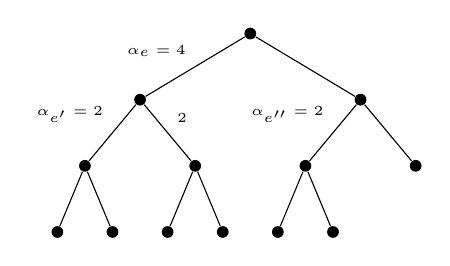
\begin{tikzpicture}[scale=0.7]

    \node[circle, fill=black, inner sep=1.5pt] (root) at (0,0) {};
    \node[circle, fill=black, inner sep=1.5pt] (n1) at (-2,-1.2) {};
    \node[circle, fill=black, inner sep=1.5pt] (n2) at (2,-1.2) {};
    \node[circle, fill=black, inner sep=1.5pt] (n3) at (-3,-2.4) {};
    \node[circle, fill=black, inner sep=1.5pt] (n4) at (-1,-2.4) {};
    \node[circle, fill=black, inner sep=1.5pt] (n5) at (1,-2.4) {};
    \node[circle, fill=black, inner sep=1.5pt] (n6) at (3,-2.4) {};
    \node[circle, fill=black, inner sep=1.5pt] (n7) at (-3.5,-3.6) {};
    \node[circle, fill=black, inner sep=1.5pt] (n8) at (-2.5,-3.6) {};
    \node[circle, fill=black, inner sep=1.5pt] (n9) at (-1.5,-3.6) {};
    \node[circle, fill=black, inner sep=1.5pt] (n10) at (-0.5,-3.6) {};
    \node[circle, fill=black, inner sep=1.5pt] (n11) at (0.5,-3.6) {};
    \node[circle, fill=black, inner sep=1.5pt] (n12) at (1.5,-3.6) {};

    \draw (root) -- (n1) node[midway, above left] {\tiny $\alpha_e = 4$};
    \draw (root) -- (n2) ;
    \draw (n1) -- (n3) node[midway, above left] {\tiny $\alpha_{e'} = 2$};
    \draw (n1) -- (n4) node[midway, above right] {\tiny 2};
    \draw (n2) -- (n5) node[midway, above left] {\tiny $\alpha_{e''} = 2$};
    \draw (n2) -- (n6);
    \draw (n3) -- (n7);
    \draw (n3) -- (n8);
    \draw (n4) -- (n9);
    \draw (n4) -- (n10);
    \draw (n5) -- (n11);
    \draw (n5) -- (n12);
    \end{tikzpicture}
    \caption{Example of the inductive step in Lemma \ref{lem:caterpillar_maximize_increasing_sums}}
    \label{fig:inductive_step_case_b}
    \end{figure}
    % end fig
\end{proof}

\subsection{The Caterpillar Bipartition Cover Bound}
\label{sec:caterpillar-bipartition-cover-bound}

\noindent Lemma~\ref{lem:caterpillar_maximize_increasing_sums} immediately implies the following main bound.

% Main Theorem %%%%%%%%
\begin{theorem}
\label{thm:caterpillar_bound}
    Suppose $h: \N \to [0,1]$ is decreasing and $\P(E_{i,1}) \geq h(\alpha_i)$. Then
%
\begin{equation}
    n_h := \inf\left\{n \in \N : \sum_{\ell=2}^{k-2}\left[1-h(\ell)\right]^n \leq 1-q\right\}
    \label{eqn:caterpillar_bound_formula}
\end{equation}
%
\noindent satisfies $N_{\mathrm{cov}}(q;\cT^*)\leq n_h$.
\end{theorem}

\begin{proof}
By the union bound and independence of the gene trees,
\[
1-\P(E_n)
\leq \sum_{i=1}^{k-3} \bigl(1-\P(E_{i,n})\bigr)
= \sum_{i=1}^{k-3} \Big[1-\P(E_{i,1})\Big]^n
\leq \sum_{i=1}^{k-3} \Big[1-h(\alpha_i)\Big]^n.
\]
Since $h$ is decreasing and bounded in $[0,1]$, the function
$f(x)=[1-h(x)]^n$ is increasing. Applying
Lemma~\ref{lem:caterpillar_maximize_increasing_sums} to this $f$ gives
\[
\P(E_n) \geq 1-\sum_{\ell=2}^{k-2}\Big[1-h(\ell)\Big]^n.
\]
Thus, for every $n$ in the set defining $n_h$, we have
$\P(E_n)\geq q$, and hence $N_{\mathrm{cov}}(q;\cT^*)\leq n_h$.
\end{proof}

\noindent If $h$ is independent of the species tree topology,
then so is equation~\eqref{eqn:caterpillar_bound_formula}. Letting
$h(x) = g_{x,1}(T_{\mathrm{min}}) \in [0,1]$, which is decreasing by
Corollary~\ref{corr:g_i1_is_decreasing}, then Theorem~\ref{thm:caterpillar_bound} and the
original bound $\P(E_{i,1}) \geq g_{\alpha_i,1}(T_{\mathrm{min}})$
of \citet{uricchio2016_bipartition_cover} give a new topology-free bound.

% Caterpillar Bound %%%%%%%
\begin{corollary}[Caterpillar Bipartition Cover Bound]
\label{cor:improved_bipartition_cover_bound_caterpillar}
\begin{equation}
    M_c(k, T_{\mathrm{min}}):=  \inf\left\{n \in \N : \sum_{\ell=2}^{k-2}\left[1-g_{\ell,1 }(T_{\mathrm{min}})\right]^n \leq 1-q\right\}
    \label{eqn:caterpillar_bound_eqn}
\end{equation}
%
\noindent satisfies $N_{\mathrm{cov}}(q;\cT^*)\leq M_c(k,T_{\mathrm{min}})$.
\end{corollary}

\noindent As with the original bound~\eqref{eqn:uricchios_bipartition_cover_bound}, equation~\eqref{eqn:caterpillar_bound_eqn}
depends on $\cT^*$ only through $k$ and $T_{\mathrm{min}}$. Heuristically, this
replaces the worst-case $g_{k-2, 1}(T_{\mathrm{min}})$ with the corresponding
order-$n$ power mean of $\{g_{\ell, 1}(T_{\mathrm{min}})\}_{\ell = 2}^{k-2}.$

% Balanced bound %%%%%%%%%%%%%%%%%%%%%%%%%%%%%%%%%%%%%%%%%%%%%%%%%%%%%%%%%%%%
\section{The Balanced-Tree Bound}
\label{sec:balanced-tree-bound}

\subsection{Coalescence Below an Edge}
\label{sec:coalescent-events-below-edge}

Theorem \ref{thm:caterpillar_bound} suggests another avenue for improvement is to
obtain a tighter bound $\P(E_{i,1}) \geq h(\alpha_i)$ than the original $h(x) = g_{x,1}(T_{\mathrm{min}})$.
For small values of $T_{\mathrm{min}}$ the bound in Corollary~\ref{cor:improved_bipartition_cover_bound_caterpillar}
is dominated by the terms $g_{\alpha_i,1}$ for which $\alpha_i$ are quite large. These are the bipartitions
 corresponding to edges $e$ close to the root of the tree which have many descendants. In \citet{uricchio2016_bipartition_cover},
 the authors essentially assume \textit{none} of the descendants coalesce before they reach edge $e$.
 When $e$ is far from the leaves, descendants have a long distance to travel through
 the tree and potentially coalesce, making this estimate very conservative.

Hence to improve this bound we should try to account for coalescent events that occur
below the edge $e$. Namely, we ought to somehow replace $g_{\alpha_e,1}(T_{\mathrm{min}})$
by $\E g_{X_e, 1}(T_{\mathrm{min}})$ where $X_e$ is the (random) number of remaining lineages
entering edge $e$. Clearly $\P(E_{i,1}) \geq \E g_{X_{e_i}, 1}(T_{\mathrm{min}})$ by the same
logic that Theorem \ref{thm:uricchios_bipartition_cover_bound} employs. In general, $X_e$ depends on
the topology of $\cT^*$ below the edge $e$. To develop a topology-free bound,
we must somehow identify the worst-case topology in this setting.

Recall a random variable $X$ is said to \textit{first-order stochastically dominate} $Y$
if $\P(X > t) \geq \P(Y > t)$ for all $t$, or equivalently if $\E u(X) \geq \E u(Y)$ for all nondecreasing
functions $u$. We denote this by $X \geq_{st} Y$. Similarly, $X$ is said to \textit{second-order stochastically dominate}
$Y$ if $\E u(X) \geq \E u(Y)$ for all nondecreasing concave functions, and we denote this
by $X \geq_{sst} Y$. First-order stochastic dominance naturally implies second-order.

 Since $x \mapsto g_{x,1}(T)$ is decreasing, convex (Corollary \ref{corr:g_i1_is_decreasing},
 Lemma~\ref{lem:g_i1_is_convex}), we see
\begin{lemma}
\label{lem:bounding_prob_with_second_order_stochastic_dominance}
If $U_{e_i} \geq_{sst} X_{e_i}$ then $\P(E_{i,1}) \geq \E g_{U_{e_i}, 1}(T_{\mathrm{min}})$.
\end{lemma}

\begin{remark}
    If $U_e$ is a function of $\alpha_e$ alone and is (second order) stochastically increasing in this parameter,
    applying Theorem~\ref{thm:caterpillar_bound} with $h(\ell) = \E g_{U_\ell, 1}(T_{\mathrm{min}})$ yields
    a new topology-free bound.
\end{remark}

 To apply this observation, we begin by analyzing the coalescent events
occurring in the two edges directly below $e$.

Let $Z_i^T$ be the random variable with distribution
 $\P(Z_i^T = j) = g_{ij}(T)$. Namely, if we start $i$ lineages then $Z_i^T$ represents the (random)
 number of lineages that remain uncoalesced after running Kingman's coalescent
 for time $T$. When we drop the $T$ superscript, it is implicitly assumed that $T = T_{\mathrm{min}}$.
 For a positive integer-valued random variable $A$, let $Z_A^T$ denote the independent mixture
 %
    \[\P(Z_A^T = i) = \sum_{\ell \geq 1} \P(A = \ell) \P(Z_\ell^T = i).\]
 %
 \noindent When we write expressions such as $Z_A^T + Z_B^T$ including multiple such mixtures,
 we implicitly mean we are mixing two independent families $\{Z_\ell\}_{\ell \geq 1}, \{Z_\ell'\}_{\ell\geq 1}$ so
 %
    \[\P(Z_A^T + Z_B^T = i) = \sum_{m=1}^{i-1} \P(Z_A^T = m) \P(Z_B^T = i-m).\]
 %
\noindent Several basic properties of these random variables and their stochastic orderings are collected
in Appendices~\ref{app:first-order-stochastic-dominance} and \ref{app:likelihood-ratio-ordering}.

Suppose below the edge $e$ our tree splits into two subtrees of size $m, k-m$. Clearly then
%
\[X_e \leq_{st}  Z_{m}^{T_1} + Z_{k-m}^{T_2},\]
%
\noindent where $T_1, T_2$ are the lengths of the branches connecting the two subtrees
to $e$.  Moreover
%
    \[Z_{m}^{T_1} + Z_{k-m}^{T_2} \leq_{st} Z_m^{T_{\mathrm{min}}} + Z_{k-m}^{T_{\mathrm{min}}},\]
%
\noindent by Lemma~\ref{lem:cdf_of_Zi}. Figure~\ref{fig:coalescent_tree} illustrates the setup. Next,
we show more balanced splits $(m, k-m)$ tend to have less coalescence.

% Coalescent tree figure
\begin{figure}[t!]
\centering
\begin{tikzpicture}[scale=1]

% Define coordinates
\coordinate (root) at (0, 3);
\coordinate (left_child) at (-1.5, 1.5);
\coordinate (right_child) at (1.5, 1.5);

% Draw the main edge e (vertical line from root)
\draw[thick] (root) -- (0, 4);
\node at (0.3, 3.5) {$e$};

% Draw branches to left and right subtrees (stopping at ellipse boundaries)
\draw[thick] (root) -- (-1.5, 2.25);
\draw[thick] (root) -- (1.5, 2.25);

% Draw the left subtree (oval containing m)
\node[draw, ellipse, minimum width=2cm, minimum height=1.5cm, thick] at (left_child) {};
\node at (left_child) {$m$};

% Draw the right subtree (oval containing k-m)
\node[draw, ellipse, minimum width=2cm, minimum height=1.5cm, thick] at (right_child) {};
\node at (right_child) {$k-m$};

% Add T_min labels positioned to the side of the branches
\node at (-1.4, 2.7) {$T_{\mathrm{min}}$};
\node at (1.3, 2.7) {$T_{\mathrm{min}}$};

\end{tikzpicture}
\caption{Coalescent tree structure showing edge $e$ with two subtrees of sizes $m$ and $k-m$. The subtrees are connected to $e$ via a branch with minimal length $T_{\mathrm{min}}$.}
\label{fig:coalescent_tree}
\end{figure}


\subsection{Deterministic Local Balancing}
\label{sec:deterministic-local-balancing}

\begin{lemma}[Deterministic Balancing Lemma]
\label{lem:deterministic_balancing_lemma} Let $k$ and $T$ be fixed. Then
    \[\quad Z^T_{i} + Z^T_{k-i} \leq_{st}  Z^T_{j} + Z^T_{k-j}, \quad\forall 1 \leq i \leq j \leq \frac{k}{2}.\]
    %
    \noindent In particular, the stochastic maximizer is $i = \lfloor k/2\rfloor$.
\end{lemma}

Heuristically, $i = \lfloor k/2 \rfloor$, where the two subtrees in Figure~\ref{fig:coalescent_tree} are as evenly
balanced as possible, is the maximizer because it minimizes the total number of pairs $\binom{m}{2} + \binom{k-m}{2}$
available in the two subpopulations, hampering coalescence. Lemma~\ref{lem:deterministic_balancing_lemma} implies
%
\begin{equation}
    X_e \leq_{st}  Z_{\lfloor \alpha_e/2 \rfloor} + Z_{\lceil \alpha_e/2 \rceil}
    \label{eqn:local-balancing-Xe-upper-bound}
\end{equation}

\begin{proof}[Proof of Lemma \ref{lem:deterministic_balancing_lemma}]
The statement is vacuously true for $k=2,3$, so for induction assume it is true for all $k' < k$. Let $S_{k,m}^T := Z_m^T + Z^T_{k-m}$ denote the total number of lineages entering an edge $e$ with subtrees of size $m,k-m$, the setup in Figure \ref{fig:coalescent_tree}. Let $\tau_{k,m}$ be the time of the first coalescent event in either of our two subpopulations of size $m,k-m$, allowing the possibility $\tau_{k,m} > T$.

The basic idea is that if we start with $k$ lineages, we can reduce to $k-1$ lineages by just waiting for the first coalescence event to occur in either subpopulation. There is of course the chance no coalescent event occurs, so we must handle this separately. The proof then relies on a few main ideas. Firstly, for more balanced splits we tend to wait longer until the first coalescent event.
\begin{proofclaim}
\label{claim:even_split_waits_longest_for_first_coalescent}
For fixed $k$, $\tau_{k,m}$ is stochastically increasing in $m$ for $1 \leq m \leq k/2$.
\end{proofclaim}

\noindent Next, conditional on a specific first coalescent time, the more balanced our split is, the more lineages tend to remain uncoalesced by the end of the branch.
\begin{proofclaim}
\label{claim:cond_first_coalescent_even_split_dominates}
For fixed $k, x,t$, $\P(S_{k,m}^T \geq x \; | \; \tau_{k,m} = t)$ is an increasing function of $m$ for $1 \leq m \leq k/2$.
\end{proofclaim}

\noindent Lastly, the more time we wait until the first coalescent event, the less time the remaining lineages have to coalesce and the more lineages we tend to have by the end of the branch.
\begin{proofclaim}
\label{claim:more_time_to_coalesce_is_better}
For fixed $k, x, m$, $\P(S_{k,m}^T \geq x \; | \; \tau_{k,m} = t)$ is an increasing function of $t$.
\end{proofclaim}

\noindent To prove Claim~\ref{claim:even_split_waits_longest_for_first_coalescent}, let $h_{k,m} := \binom{m}{2} + \binom{k-m}{2}$.
Then $\tau_{k,m} \sim \mathrm{Exp}\left(h_{k,m}\right)$. Since
\[
\P(\tau_{k,m} > t) = \exp\left(-th_{k,m}\right)
\]
and $h_{k,m}$ is decreasing in $m$ for $1 \leq m \leq k/2$, these tails are increasing
in $m$. Hence $\tau_{k,m}$ is stochastically increasing in $m$ as desired.


 To prove Claim~\ref{claim:cond_first_coalescent_even_split_dominates}, first suppose $t > T$. No coalescent event occurs before time $T$, so
\[
\P(S_{k,m}^T \geq x \mid \tau_{k,m}=t)=\ind\{x\leq k\},
\]
which is independent of $m$, so the claim is trivial. For $t \leq T$, by the strong
memoryless property of the exponential distribution underlying Kingman's coalescent, we know
\begin{equation}
\P(S_{k,m}^T \geq x \; | \; \tau_{k,m} = t) = p_{k,m} \cdot \P(S_{k-1,m-1}^{T-t} \geq x) + (1-p_{k, m}) \cdot \P(S_{k-1,m}^{T-t} \geq x),
\label{eqn:split_on_first_coalescent_event}
\end{equation}
where
\[
p_{k,m} = \frac{\binom{m}{2}}{\binom{m}{2} + \binom{k-m}{2}}
\]
is the probability the first coalescence occurs in the population of size $m$.
Namely, after the first coalescent event occurs in either subpopulation, what remains
is a Kingman's coalescent with one less lineage. For $1 \leq m \leq k/2 - 1$, by induction
\begin{align*}
& \P(S_{k,m}^T \geq x \; | \; \tau_{k,m} = t)\\
&= p_{k,m} \cdot \P(S_{k-1,m-1}^{T-t} \geq x) + (1-p_{k, m}) \cdot \P(S_{k-1,m}^{T-t} \geq x) \\
&\leq \P(S_{k-1,m}^{T-t} \geq x) \\
&\leq p_{k,m+1} \cdot \P(S_{k-1,m}^{T-t} \geq x) + (1-p_{k, m+1}) \cdot \P(S_{k-1,m+1}^{T-t} \geq x)\\
&= \P(S_{k,m+1}^T \geq x \; | \; \tau_{k,m+1} = t).
\end{align*}
Thus $\P(S_{k,m}^T \geq x \; | \; \tau_{k,m} = t)$ is increasing in $m$ for each fixed $t$.

 To prove Claim~\ref{claim:more_time_to_coalesce_is_better}, by equation~\eqref{eqn:split_on_first_coalescent_event} it suffices
 to show for fixed $k,m$ that $S^T_{k,m}$ is stochastically decreasing in $T$. But this follows from a
 simple coupling argument. For $s \leq T$, couple $S_{k,m}^T$ to $S_{k,m}^s$ by using the same
 exponential clocks for the coalescent events. At time $s$ the number of lineages
 remaining agree, and $S^T_{k,m}$ can only decrease from here if more coalescents
  occur between times $s$ and $T$.

With the claims proved, we are ready to finally finish our proof of
Lemma \ref{lem:deterministic_balancing_lemma}. Note that our above claims are exactly the
conditions of the Mixture Lemma (Lemma~\ref{lem:mixtures_and_stochastic_dominance}), which shows first-order 
stochastic dominance is preserved by increasing mixtures, where $\{S_{k,m}^T\}_{m=1}^{\lfloor k/2\rfloor}$ are playing the
role of our $V_i$ and $\{\tau_{k,m}\}_{m=1}^{\lfloor k/2\rfloor}$ are playing the role of our $\Theta_i$.
Hence the result just follows from applying this lemma.
\end{proof}

%%%%%%%%%%%%%%%%%%%%%%%%%%%%%%%%%%%%%%%%%%%%
% Recursive balancing %%
%%%%%%%%%%%%%%%%%%%%%%%%%%%%%%%%%%%%%%%%%%%%
\subsection{Recursive Balancing and the Balanced Worst Case}
\label{sec:recursive-balancing}

By iterating the ideas from the previous section, it is natural to believe the topology
minimizing coalescence is the one where \textit{all} splits are even, namely when the
topology below edge $e$ is the balanced tree. This is true in the following sense.

Given a binary tree $\cT$ (with branch lengths) let $X_\cT$ denote the number of
lineages that have not coalesced by the time they reach the root. We first prove
an extension of our deterministic balancing lemma,
Lemma~\ref{lem:deterministic_balancing_lemma}, which allows
for random subpopulations.

To do so, we require a slightly stronger stochastic order than $\leq_{st}$. We say a random variable $X$ is less than $Y$ with respect to the
\emph{likelihood ratio ordering (LRO)}, and write $X\leq_{lr}Y$, if the
likelihood ratio $f_Y(t)/f_X(t)$ is nondecreasing in $t$, where $f_X$ and
$f_Y$ are the respective mass functions. Equivalently,
\[
f_X(s)f_Y(t) \geq f_X(t)f_Y(s), \qquad s\leq t.
\]
The LRO implies first-order stochastic dominance.

% Balancing Lemma %%%%%%%%%%%%
\begin{lemma}[Balancing Lemma]
\label{lem:balancing_lemma}
If $A,A', B, B'$ are mutually independent, non-negative integer-valued random variables
so that $A \leq_{lr} A'$ and $B \leq_{lr} B'$, then
%
\[Z_{A + B} + Z_{A' + B'} \leq_{st} Z_{A + B'} + Z_{A' + B}. \]
\end{lemma}
%
\noindent Note when $A,B,A', B'$ are all deterministic, this reduces to Lemma \ref{lem:deterministic_balancing_lemma}.

\begin{proof}[Proof of Balancing Lemma \ref{lem:balancing_lemma}]
    First observe that for a fixed sum $s$, the deterministic balancing Lemma~\ref{lem:deterministic_balancing_lemma} implies the random variables
    %
    \[Y_d := Z_{\frac{s+d}{2}} + Z_{\frac{s-d}{2}}\]
    %
    \noindent are decreasing with respect to $\leq_{st}$ for $0 \leq d < s$. By the Mixture Lemma (Lemma~\ref{lem:mixtures_and_stochastic_dominance}),
    we see $Y_{D} \geq_{st} Y_{D'}$ whenever $0 \leq D \leq_{st} D' < s$. Namely, if we fix the total number of lineages $s$,
    then if the imbalance $D$ between our two subpopulations tends to be less than imbalance $D'$, we tend
    to have less coalescence.

    From here, the idea is simple: we condition on the total number of lineages across the two populations, and attempt
    to control the conditional differences. For convenience, define
    %
    \[\Delta_A := A' - A, \quad \Delta_B := B' - B, \quad S_A := A' + A, \quad S_B = B' + B.\]
    %
    Now, note in both $Z_{A + B} + Z_{A' + B'}$ and $Z_{A + B'} + Z_{A' + B}$ the total number of
    lineages $S = S_A + S_B$ is the same. Hence, by conditioning on $S_A,S_B, |\Delta_A|,$ and $|\Delta_B|$, it suffices to show $D' \geq_{st} D$,
    where $D,D'$ are the conditional differences
    %
    \[D' = |\Delta_A + \Delta_B| \mid \{|\Delta_A|, |\Delta_B| , S_A, S_B \}, \qquad D = |\Delta_A - \Delta_B| \mid \{|\Delta_A|, |\Delta_B| , S_A, S_B \}.\]
    %
    \noindent After this conditioning, $\{D, D'\} = \{|\Delta_A| + |\Delta_B|, ||\Delta_A| - |\Delta_B||\}$. If $|\Delta_A|=0$ or $|\Delta_B|=0$, then $D=D'$, and the conclusion is immediate. Hence suppose both absolute differences are positive. Let

    \[q = \P(D' = |\Delta_A| + |\Delta_B|) = \P(\Delta_A\Delta_B \geq 0 \mid |\Delta_A|, |\Delta_B| , S_A, S_B)\]

    \noindent be the probability $D'$ takes on the larger of these two values. Then it suffices to show $q \geq 1/2$. Since $\Delta_A, \Delta_B$ are conditionally independent given $S_A, S_B$
    %
    \[q = p_Ap_B + (1-p_A)(1-p_B) \geq \frac{1}{2} \iff \left(p_A - \frac{1}{2} \right) \left(p_B - \frac{1}{2} \right) \geq 0,\]
    %
    \noindent where $p_A = \P(\Delta_A \geq 0 \mid |\Delta_A|, S_A)$ and likewise for $p_B$. We will show that $p_A, p_B \geq 1/2$, completing the proof. Note conditional on $\{|\Delta_A| = m, S_A = s\}$ then $p_A \geq 1/2$ occurs precisely when
    %
    \[\P\left(A'=\frac{s+m}{2}, A = \frac{s-m}{2}\right) \geq \P\left(A'=\frac{s-m}{2}, A = \frac{s+m}{2}\right).\]
    %
    \noindent As $A,A'$ are independent, this follows from $A \leq_{lr} A'.$ Similarly, $p_B \geq 1/2$, so $D' \geq_{st} D$. The result
    follows then by taking expectations with respect to $\Delta_A, \Delta_B, S_A, S_B$.
\end{proof}

With the random balancing lemma in hand, we can now iterate local balancing
through the tree. This shows that the balanced topology minimizes coalescence
among all trees with the same number of leaves. The following result makes this
precise.

% Balanced is worst case
\begin{lemma}[Balanced Tree Is Worst Case]
\label{lem:balanced_is_worse_case}
    If $\cB_k$ is the balanced tree with $k$ leaves and all branch lengths
    equal to $T_{\mathrm{min}}$ then $X_{\cB_k} \geq_{st} X_\cT$ for any other
    tree $\cT$ with $k$ leaves and minimum branch length $T_{\mathrm{min}}$.
\end{lemma}

\begin{proof}[Proof of Lemma \ref{lem:balanced_is_worse_case}]
First, by a simple coupling argument we see replacing every branch length in $\cT$ by $T_{\mathrm{min}}$ can only
increase the number of lineages reaching the root. It therefore suffices to
assume that all branch lengths are $T_{\mathrm{min}}$.

Throughout the proof, write $X_r:=X_{\cB_r}$ and $U_r:=Z_{X_r}$, with all
occurrences of these random variables understood to be independent copies when
they arise from disjoint subtrees. Define $X_0 = U_r := 0$. We first establish the balanced-subtree split
comparison
%
\begin{equation}
U_m+U_{k-m}
\leq_{st}
U_{\lfloor k/2\rfloor}+U_{\lceil k/2\rceil} \overset{d}{=} X_k,
\qquad 1\leq m\leq\lfloor k/2\rfloor.
\label{eq:balanced-subtree-split-comparison}
\end{equation}
%
The idea of the proof is simple: $X_m$ and $X_{k-m}$ consist of two subtrees of
size (approximately) $m/2$ and $(k-m)/2$ respectively. By taking one subtree from each of $X_m, X_{k-m}$ and swapping them 
using the balancing lemma~\ref{lem:balancing_lemma}, we balance these two subpopulations so they are both (approximately) size $k/2$. 
From there, we can inductively balance these two subpopulations separately to get the result.

More formally, we prove equation~\eqref{eq:balanced-subtree-split-comparison} by strong induction
on $k$. The cases $k\leq3$ are
immediate. For $k=4$, the only nontrivial comparison is
\[
U_1+U_3=Z_1+Z_{X_3}
\leq_{st} Z_1+Z_3
\leq_{st} Z_2+Z_2
=U_2+U_2,
\]
where the first inequality follows from Corollary~\ref{corollary:stochastic_dominance_composition}
because $X_3\leq3$ almost surely, and the second from the deterministic balancing lemma,
Lemma~\ref{lem:deterministic_balancing_lemma}.

Now suppose equation~\eqref{eq:balanced-subtree-split-comparison}
holds for every $k'<k$, and fix $1\leq m < \lfloor k/2\rfloor$. Set
\[
a=\lfloor m/2\rfloor,\qquad a'=\lceil m/2\rceil,\qquad
b=\lfloor(k-m)/2\rfloor,\qquad b'=\lceil(k-m)/2\rceil.
\]
Then $a\leq a'\leq b\leq b'$, and the recursive construction of the balanced
trees gives
\[
X_m\stackrel{d}{=}U_a+U_{a'},
\qquad
X_{k-m}\stackrel{d}{=}U_b+U_{b'}.
\]
Since $U_r$ is increasing in the likelihood-ratio order (Lemma~\ref{lem:xi_zxi_increasing_in_lro}),
\[
U_a\leq_{lr}U_{a'}\leq_{lr}U_b\leq_{lr}U_{b'}.
\]

Suppose first that $k$ is even. Since
$a+b'=a'+b=k/2$, apply the Balancing Lemma with
$(A,A',B,B')=(U_a,U_b,U_{a'},U_{b'})$ to obtain
%
\begin{equation*}
U_m+U_{k-m} \stackrel{d}{=}Z_{U_a+U_{a'}}+Z_{U_b+U_{b'}} \leq_{st}Z_{U_a+U_{b'}}+Z_{U_{a'}+U_b}.
\end{equation*}
%
Applying the inductive hypothesis with total $k/2$ shows both $U_a + U_{b'} \leq_{st} X_{k/2}$ and $U_{a'} + U_b \leq_{st} X_{k/2}$.
As $U \mapsto Z_U$ preserves $\leq_{st}$ by Corollary~\ref{corollary:stochastic_dominance_composition}, we see
\[
U_m+U_{k-m}
\leq_{st}Z_{X_{k/2}}+Z_{X_{k/2}}
=U_{k/2}+U_{k/2},
\]
which proves equation~\eqref{eq:balanced-subtree-split-comparison} for even $k$.

If $k$ is odd, then
$a+b=(k-1)/2$ and $a'+b'=(k+1)/2$. Applying the Balancing Lemma with
$(A,A',B,B')=(U_a,U_{b'},U_{a'},U_b)$ gives
%
\begin{equation*}
    U_m+U_{k-m}\stackrel{d}{=}Z_{U_a+U_{a'}}+Z_{U_b+U_{b'}}\leq_{st}Z_{U_a+U_b}+Z_{U_{a'}+U_{b'}}.
\end{equation*}
%
The inductive comparisons with totals $(k-1)/2$ and $(k+1)/2$ bound
the two inner sums by $X_{(k-1)/2}$ and $X_{(k+1)/2}$, respectively. Therefore
\[
U_m+U_{k-m}
\leq_{st}Z_{X_{(k-1)/2}}+Z_{X_{(k+1)/2}}
=U_{\lfloor k/2\rfloor}+U_{\lceil k/2\rceil}.
\]
This completes the proof of the balanced-subtree split comparison.

We now prove the stated worst-case result, again by induction on $k$. The case $k=1$
is immediate. Suppose the result holds for every smaller tree, and let $L$ and
$R$ be the two root subtrees of $\cT$, with $m$ and $k-m$ leaves, respectively,
where $m\leq k-m$. The inductive hypothesis gives
$X_L\leq_{st}X_m$ and $X_R\leq_{st}X_{k-m}$. Consequently,
Corollary~\ref{corollary:stochastic_dominance_composition} and
equation~\eqref{eq:balanced-subtree-split-comparison} give
\[
X_\cT
=Z_{X_L}+Z_{X_R}
\leq_{st}U_m+U_{k-m}
\leq_{st}U_{\lfloor k/2\rfloor}+U_{\lceil k/2\rceil}
=X_{\cB_k}.
\]
\end{proof}

\subsection{The Balanced Bipartition Cover Bound}
\label{sec:balanced-bipartition-cover-bound}

Lemma \ref{lem:balanced_is_worse_case} suggests a natural way of upper-bounding
the number of lineages $X_e$ entering a given edge $e$: $X_e \leq_{st} X_{\cB_{\alpha_e}}$. From this, we get our final bound.


% Balanced bipartition cover bound %%%%%%%%%%
\begin{theorem}[Balanced Bipartition Cover Bound]
\label{thm:improved_bipartition_cover_bound_balanced}
 Let
\begin{equation}
    M_b(k, T_{\mathrm{min}}):=  \inf\left\{n \in \N : \sum_{\ell=2}^{k-2}\left[1-w_\ell(T_{\mathrm{min}})\right]^n \leq 1-q\right\}
\label{eqn:balanced-bound}
\end{equation}
%
\noindent where $w_\ell := \P(Z_{X_{\cB_\ell}} = 1)$. Then $N_{\mathrm{cov}}(q;\cT^*)\leq M_b(k,T_{\mathrm{min}})$. In particular,
\[
N_{\mathrm{cov}}(q;\cT^*)\leq \left\lceil
    \frac{\log\!\left(\frac{k-3}{1-q}\right)}
         {-\log\!\left(1-w_{k-2}(T_{\mathrm{min}})\right)}
\right\rceil.
\]
\end{theorem}


% Proof
\begin{proof}[Proof of Theorem \ref{thm:improved_bipartition_cover_bound_balanced}]
    Lemma \ref{lem:balanced_is_worse_case} implies $X_e \leq_{st} X_{\cB_{\alpha_e}}$
    so by the remark below Lemma \ref{lem:bounding_prob_with_second_order_stochastic_dominance} it
    suffices to show that $U_\ell := X_{\cB_\ell}$ is stochastically increasing in $\ell$. This follows from
    induction as
    %
        \[U_\ell \overset{d}{=} Z_{U_{\lfloor \ell/2 \rfloor}} + Z'_{U_{\lceil \ell/2 \rceil}}.\]
    %
    \noindent When $\ell$ increases by one, exactly one of $\lfloor \ell/2\rfloor$ and
    $\lceil \ell/2\rceil$ increases by one. Hence the inductive hypothesis and
    Corollary~\ref{corollary:stochastic_dominance_composition} imply
    $U_{\ell+1} \geq_{st} U_\ell$. It follows that
    \[
        h(\ell):=\E g_{U_\ell,1}(T_{\mathrm{min}})=w_\ell(T_{\mathrm{min}})
    \]
    is decreasing. Applying Theorem~\ref{thm:caterpillar_bound} with this choice of
    $h$ gives the first bound. Moreover,
    $w_\ell(T_{\mathrm{min}})\geq w_{k-2}(T_{\mathrm{min}})$ for
    $2\leq\ell\leq k-2$, so
    \[
    \sum_{\ell=2}^{k-2}\left[1-w_\ell(T_{\mathrm{min}})\right]^n
    \leq (k-3)\left[1-w_{k-2}(T_{\mathrm{min}})\right]^n.
    \]
    Solving the resulting inequality for $n$ gives the stated explicit bound.
\end{proof}
% end proof

\noindent As the subtrees of a balanced tree are balanced, we can calculate $w_\ell(T_{\mathrm{min}})$ easily
in a recursive fashion. Letting $W_\ell := Z_{X_{\cB_\ell}}$, we see $W_1 \equiv 1$ and
$W_\ell =^d Z_{W_{\lfloor \ell/2 \rfloor} + W_{\lceil \ell/2 \rceil}}$, so
%
\begin{equation}
    \P(W_\ell=j)
    =
    \sum_{a\geq 1}\sum_{b\geq 1}
    \P\left(W_{\lfloor\ell/2\rfloor}=a\right)
    \P\left(W_{\lceil\ell/2\rceil}=b\right)
    g_{a+b,j}(T_{\mathrm{min}}),
    \qquad \ell\geq 2.
    \label{eqn:balanced-W-recursion}
\end{equation}

%%%%%%%%%%%%%%%%%%%%%%%%%%%%%%%%%%%%%%%%%%%%%%%%
% Asymptotic analysis
%%%%%%%%%%%%%%%%%%%%%%%%%%%%%%%%%%%%%%%%%%%%%%%%
\section{Asymptotic Growth and Improvement Factors}
\label{sec:asymptotic-growth}

 Since the bounds are complicated functions of $T_{\mathrm{min}}$ and $k$, we develop estimates
 of their scaling with respect to these two parameters.

 Here we confirm our intuition that our new bounds drastically improve performance
 in the small $T$ regime. For fixed $T$, we show that all the bounds are $\Theta_T(\log(k))$, and that
 this is essentially the best one can do while relying on the union bound. We start with a
 result that specifies the asymptotics of the function $g_{k,1}(T)$ underlying all our bounds.

\subsection{Coalescence-Probability Asymptotics}
\label{sec:coalescence-probability-asymptotics}

\begin{lemma}[Asymptotics of $g_{k,1}(T)$]
\label{lem:asymptotics_g_k1(T)}
The function $T \mapsto g_{k,1}(T)$ has asymptotics
\begin{equation}
     \begin{cases} 1 - g_{k,1}(T) \sim \frac{3(k-1)}{k+1} \exp(-T), & T \uparrow \infty, \\
 g_{k,1}(T) \sim \frac{k!}{2^{k-1}} T_k^{k-1}, &  k^2T_k = o(1).
\end{cases}
\label{eqn:asymptotics_T_mapsto_g_k1(T)}
\end{equation}
\noindent Moreover, for fixed $T$, we have $g_{k,1}(T) \downarrow \P(S_\infty \leq T) =: s(T)$ where $S_\infty := \sum_{i=2}^\infty \tau_i$ for $\tau_i \sim \mathrm{Exp}\left(\binom{i}{2}\right)$ independent. Furthermore, the gap $\Delta_k(T) := g_{k,1}(T) - s(T)$ satisfies
%
\[\Delta_k(T) = \frac{2f_{S_\infty}(T)}{k} + o\left(\frac{1}{k}\right) \sim \frac{2f_{S_\infty}(T)}{k}.\]
%
\end{lemma}

\noindent The proof can be found in Appendix~\ref{app:coalescent-asymptotics-proof}.

\subsection{Asymptotic Growth of the Bounds}
\label{sec:asymptotic-bound-growth}

Using this, we develop the following asymptotics for our two bounds. Recall
that $M_o(k,T)$ denotes the original bound of \citet{uricchio2016_bipartition_cover} and $M_b(k,T)$
our balanced bound (Theorem~\ref{thm:improved_bipartition_cover_bound_balanced}). Let
%
    \[u(T) := \frac{2-\exp(-T/2)}{1-\exp(-T/2)} \geq \E X_{\cB_k}^T\]
%
\noindent be our upper bound on the number of lineages reaching the root
of a balanced tree, which we prove in Corollary~\ref{corr:upperbound_lineages_balanced} below.

Jensen's inequality then gives the convenient upper bound
%
\[M_b(k,T) \leq \frac{\log\left(\frac{k-3}{1-q}\right)}{-\log\left(1-g_{\E X_{\cB_{k-2}}, 1}(T)\right)}.\]
%
Thus the balanced-tree analysis replaces $k-2$ by $\E X_{\cB_{k-2}}$, which may be
substantially smaller.

\begin{lemma}[Bound Asymptotics]
\label{lem:bound_asymptotics}
    Let $\kappa_{q,k} := \log((k-3)/(1-q))$. Then
    %
    \[M_o(k,T)  \sim \begin{cases}
    \frac{\kappa_{q,k}}{T}, & T \uparrow \infty, \\
    \frac{2^{k-3}\kappa_{q,k}}{(k-2)! T^{k-3}}, & T = o(k^{-2}), \\
    \frac{\kappa_{q,k}}{-\log(1-s(T))}, & T \text{ fixed}, k \to \infty
\end{cases}\]

    \[M_b(k,T) \lesssim
        \frac{\kappa_{q,k}}{-\log(1-g_{u(T), 1}(T))}, \qquad T \text{ fixed}, k \to \infty\]

\end{lemma}

\begin{proof}
Let $s(T) := \P(S_\infty \leq T)$ be our limiting CDF,
$\Delta_k(T) := g_{k,1}(T) - s(T)$ our gap, and
$c(T) := 2f_{S_\infty}(T)$ our gap's asymptotic constant.

We start with $M_o$. Note Lemma \ref{lem:asymptotics_g_k1(T)} implies
%
\begin{equation}
    \log(1-g_{k,1}(T)) \sim \begin{cases} - T, & T \uparrow \infty, \\
 -\frac{k!}{2^{k-1}} T^{k-1}, &  T = o(k^{-2}).
\end{cases}
\label{eqn:asymptotics_T_mapsto_log(one_minus_g_k1(T))}
\end{equation}
%
\noindent From this

\[M_{o}(k,T) \sim \begin{cases}
    \frac{\kappa_{q,k}}{T}, & T \uparrow \infty, \\
    \frac{2^{k-3}\kappa_{q,k}}{(k-2)! T^{k-3}}, & T = o(k^{-2}).
\end{cases}\]

\noindent In particular, we recover the small $T$ bound found in Appendix $B$ of \cite{shekhar2018_how_many_genes_are_enough}, although here we exactly quantify the asymptotic constant.

For the fixed $T$ and asymptotic $k$ bound, we Taylor expand $\log(x)$ about $1 - s$ to observe
%
\[\log(1 - g_{k,1}(T) )= \log(1-s)-\sum_{n=1}^\infty \frac{\Delta^n}{n(1-s)^n} = \log(1-s) - \frac{\Delta}{1-s} - O(\Delta^2).\]
%
\noindent Hence this and Lemma \ref{lem:asymptotics_g_k1(T)} imply as $k \to \infty$
%
\[M_o(k,T) = \frac{\kappa_{q,k}}{\left(\frac{c(T)}{1-s} + o(1)\right) \cdot \frac{1}{k} - \log(1-s)} \sim \frac{\kappa_{q,k}}{-\log(1-s)}.\]

\noindent For $M_b(k,T)$, note as $g_{k,1}(T)$ is decreasing in $k$ we have
%
\[\sum_{\ell=2}^{k-2} (1-w_\ell(T))^n \geq (k-3)(1-g_{2,1}(T))^n = (k-3)\exp(-nT).\]
%
\noindent Hence $M_b(k,T)\geq \kappa_{q,k}T^{-1}$.
As $k \mapsto g_{k,1}(T)$ is decreasing and convex by Lemma \ref{lem:g_i1_is_convex},
%
\[\sum_{\ell=2}^{k-2} (1-\E g_{U_\ell, 1}(T))^n \leq (k-3) (1- g_{\E U_{k-2}, 1}(T))^n.\]
%
\noindent Applying Corollary \ref{corr:upperbound_lineages_balanced},
%
\[M_b(k,T) \leq \frac{\kappa_{q,k}}{-\log(1-g_{u(T),1}(T))}.\]
%
\noindent Combining these two previous results,
%
\[\frac{\kappa_{q,k}}{T} \leq M_{b}(k,T) \leq \frac{\kappa_{q,k}}{-\log(1-g_{u(T), 1}(T))}.\]
%
\noindent Since $M_b(k,T) \leq M_o(k,T)$, the lower bound shows us $M_b(k,T) \sim \kappa_{q,k} T^{-1}$ as $T \to \infty$. Since $u(T) \sim 2/T$ as $T \downarrow 0$, the preceding Taylor asymptotics, which require $k^2T=o(1)$, do not describe the relevant joint regime. Lemma~\ref{lem:improvement_ratio_asymptotics} analyzes this regime directly.

\end{proof}

\subsection{The Improvement Factor}
\label{sec:asymptotic-improvement-factor}

\begin{lemma}[Improvement Factor]
\label{lem:improvement_ratio_asymptotics}
For fixed $T$, the improvement factor satisfies
\[
\liminf_{k\to\infty}\frac{M_o(k,T)}{M_b(k,T)}
\geq \beta_T
:=\frac{\log(1-g_{u(T),1}(T))}{\log(1-s(T))}.
\]
Moreover, as $T\downarrow0$,
\[
\log\beta_T=\Theta(T^{-1}).
\]
\end{lemma}

\begin{proof}
The fixed-$T$ estimates in Lemma~\ref{lem:bound_asymptotics} give
\[
M_o(k,T)\sim\frac{\kappa_{q,k}}{-\log(1-s(T))},
\qquad
M_b(k,T)\lesssim
\frac{\kappa_{q,k}}{-\log(1-g_{u(T),1}(T))},
\]
which imply the stated lower bound on the limiting improvement factor.

Since $-\log(1-x)\sim x$ as $x\downarrow0$ and both
$g_{u(T),1}(T),s(T)\downarrow0$, we have
\[
\log\beta_T=\log g_{u(T),1}(T)-\log s(T)+o(1).
\]
We first control $\log s(T)$. Let
$K(x):=\log\E\exp(-xS_\infty)$. By independence, for $x>0$,
\[
K(x)=-\log\left(\prod_{n=2}^\infty
\left[1+\frac{x}{\lambda_n}\right]\right).
\]
Since $(n-1)^2\leq2\lambda_n\leq n^2$, the infinite-product expansion of
$\sinh$ gives
\[
0\leq K(x)+\log\left(\frac{\sinh(\pi\sqrt{2x})}{\pi\sqrt{2x}}\right)
\leq\log(1+2x).
\]
Thus $K(x)\sim-\pi\sqrt{2x}$ as $x\to\infty$. Applying Corollary 2 of
\cite{cadena2015_tauberian_theorems_exponential_type} with
$A=1$, $P(x)=s(x)$, $B=-\pi^2/2$, and $\beta=-1$ yields
\[
\log s(T)\sim-\frac{\pi^2}{2}T^{-1}
\qquad\text{as }T\downarrow0.
\]

Next, $\log g_{u(T),1}(T)\leq0$, which already gives
$\log\beta_T=O(T^{-1})$. For the lower bound, let
$\tau_i\sim\mathrm{Exp}(\binom{i}{2})$ be independent, so
\[
g_{k,1}(T)=\P\left(\sum_{i=2}^k\tau_i\leq T\right).
\]
Using $1-e^{-x}\geq x/(1+x)$,
\[
g_{k,1}(T)
\geq\P\left(\bigcap_{i=2}^k
\left\{\tau_i\leq\frac{T}{k-1}\right\}\right)
\geq\prod_{i=2}^k
\frac{\frac{T}{k-1}\binom{i}{2}}
{1+\frac{T}{k-1}\binom{i}{2}}.
\]
If $x_{i,T}:=\frac{T}{k-1}\binom{i}{2}$, then
\[
T\log g_{k,1}(T)
\geq Tk\cdot\frac{1}{k}\sum_{i=2}^k
\log\frac{x_{i,T}}{1+x_{i,T}}.
\]
Since $u(T)\sim2/T$, a Riemann-sum approximation gives
\[
T\log g_{u(T),1}(T)
\geq2\int_0^1\log\frac{y^2}{1+y^2}\,dy+o(1)
=-(\pi+2\log2)+o(1).
\]
Combining this with the asymptotics for $\log s(T)$ gives
\[
\log\beta_T
\geq T^{-1}\left(-\pi-2\log2+\frac{\pi^2}{2}+o(1)\right)
=\Omega(T^{-1}).
\]
Together with the upper bound, this proves
$\log\beta_T=\Theta(T^{-1})$.
\end{proof}

Thus, in this regime, the asymptotic lower bound on the improvement factor grows
exponentially in $T^{-1}$.

\subsection{Limits of the Union-Bound Framework}
\label{sec:union-bound-limitations}

Repeating the above analysis shows that \textit{any} bound built using the union bound and the coalescent function $g_{k,1}(T)$ cannot be asymptotically better than $\log(k)/T$. This is true, \textit{even if the descendant counts $\alpha_i$ are known}, as we can still upper bound $g_{\alpha_i, 1}(T) \leq g_{2,1}(T)$. Hence the asymptotics in $k$ are fundamentally limited to $\Theta(\log(k))$ by our union bound argument, and we can only hope to improve upon the constant down to the limit $T^{-1}$. The next section examines the corresponding finite-parameter improvements numerically.


To see why the $\Theta(\log(k))$ growth rate is natural for the $k$ asymptotics,
note that $g_{k,1}(T)$ is roughly constant and equal to $s(T) > 0$ for all large $k$.
Hence in large caterpillar trees, where most of the edges have large descendant counts,
most of their bipartitions have $g_{k,1}(T)$ saturating in this way.

In this setting, we are essentially saying each bipartition corresponds to
a $\mathrm{Geometric}(s(T))$ random variable which specifies how many gene trees we need
for that specific bipartition to show up. Each such variable has tail
 $\P(\mathrm{Geo}(s) > m) = (1-s)^{m}$. Solving for $p(m) = k^{-1}$ we see
 $m = \log(k)/[-\log(1-s)]$, so the maximum of $k$ independent such geometric random
 variables ought to be roughly of this order.

% Experimental Results %%%%%%%%%%%%%%%%%%%%%%%%%%%%%%%%%%%%%%%%%%%%%%%%%%%
\section{Numerical Results and Simulations}
\label{sec:simulations}

In this section we compare the performance of our new bounds both to
the original bound of \citet{uricchio2016_bipartition_cover} and to empirical
results coming from simulations of the MSC model under various species tree topologies.
Code for reproducing the below figures can be found on GitHub \citep{mcnulty2025_msc_bipartition_cover_code}.


% Bound growth rates
\subsection{Numerical Growth of the Bounds}
\label{sec:bound-growth-rates}

First, we numerically explore how the original and balanced bounds grow as functions of the two key parameters:
the minimum branch length $T_{\mathrm{min}}$ and the species count $k$. We evaluated the
bounds at coverage probability $q=0.99$, for $T_{\mathrm{min}}\in\{0.1,0.2,0.5,1,2\}$
and $k\in\{5,10,15,20,25,30\}$. Figure \ref{fig:bound_comparison} highlights our results.
Both bounds increase with $k$ and decrease with $T_{\mathrm{min}}$, as expected. However,
the balanced bound is dramatically lower in essentially all regimes.

% Bound comparisons (as functions of k, T_min)
\begin{figure}[!tbp]
    \centering
    \captionsetup{type=figure, justification=raggedright, singlelinecheck=false}
    
\includegraphics[height=4cm]{bound_plots/original_bound.png}

    
\includegraphics[height=4cm]{bound_plots/balanced_bound.png}
    \caption{Bipartition cover bounds as functions of the two key parameters $k$ and $T_{\min}$. (top) The original bound \citep{uricchio2016_bipartition_cover}. (bottom) The balanced bound (Theorem~\ref{thm:improved_bipartition_cover_bound_balanced}).}
    \label{fig:bound_comparison}
\end{figure}

While it varies species to species, the maximal number of independent genes is typically
on the order of $10^3$ to $10^5$ \cite{loman2015_bacterial_genome_sequencing, pertea2023_human_gene_catalogue}.
One drawback of the original bipartition cover bound \eqref{eqn:uricchios_bipartition_cover_bound} that
Figure \ref{fig:bound_comparison} highlights is that it dips above this threshold even for relatively
few species $k$, especially when the minimum branch length is short. This can limit its practicability
because scientists might not have access to enough genes to achieve their desired coverage probability.
One attractive feature of our new bound is that it remains below these biologically reasonable
thresholds for a much wider parameter range, greatly improving its utility.


% Improvement Ratios
\subsection{Numerical Improvement Ratios}
\label{sec:improvement-ratios}

To quantify how much these new bounds improve on the bound of \cite{uricchio2016_bipartition_cover},
we plot the ratios $I := M_{\mathrm{old}}/M_{\mathrm{new}}$ again as functions of
the two nontrivial parameters $T_{\mathrm{min}}, k$. Values of $I > 1$ indicate an improvement over the
 original bound, and values $I < 1$ a degradation. Figure \ref{fig:improvement_ratios} shows
 these improvement ratios over the same parameter range as the previous subsection.

% Improvement ratio fig
\begin{figure}[!tbp]
    \centering
    \captionsetup{type=figure, justification=raggedright, singlelinecheck=false}
    
\includegraphics[height=4cm]{improvement_ratios/cat_vs_original.png}

    
\includegraphics[height=4cm]{improvement_ratios/balanced_vs_original.png}
    \caption{Improvement ratios. (top) Improvement of the caterpillar bound (Corollary~\ref{cor:improved_bipartition_cover_bound_caterpillar}) over the original bound (Theorem~\ref{thm:uricchios_bipartition_cover_bound}). (bottom) Improvement of the balanced bound (Theorem~\ref{thm:improved_bipartition_cover_bound_balanced}) over the original bound.}
    \label{fig:improvement_ratios}
\end{figure}

 As Figure \ref{fig:improvement_ratios} highlights, most of the improvement comes from the more
 sophisticated balanced bound (Theorem \ref{thm:improved_bipartition_cover_bound_balanced}), which
 improves on the original bound by several orders of magnitude in the challenging high $k$ and
 low $T_{\mathrm{min}}$ regimes.

On the other hand, the caterpillar bound only improves by a small constant factor. This is due to
the fact
%
    \[s(T) := \lim_{\ell \to \infty} g_{\ell,1}(T) > 0,\]
%
so most terms in the  sum $\sum_{\ell=2}^{k-2} (1-g_{\ell,1}(T))^n$ quickly saturate near $s(T)$ and we
gain little by replacing the maximum $g_{k-2,1}(T)$ by $g_{\ell, 1}(T)$.


% Empirical Comparison
\subsection{Simulation-Based Overestimation}
\label{sec:quantifying-overestimation}

In this subsection, we aim to quantify the level to which our bounds
overestimate the number of gene trees required to obtain a bipartition cover.
If $n_b$ is one of our upper bounds, define the \textit{overestimation ratio} to be the
quantity $n_b/N_{cov}(q; \cT^*)$. To estimate $N_{cov}(q; \cT^*)$, we sample gene
trees independently from the MSC model until we get a bipartition cover, and repeat
this for $N$ independent trials to get an estimate of the desired
quantile. We used $N=10^4$ and $q=0.9$. These were chosen so a significant
number of trials (roughly $1000$) would generate data above the true $90^{th}$ quantile.
Each trial was capped at $10^5$ gene trees, and we required fewer than $1\%$ of trials in every
parameter setting to reach this cap.

We explore a few different species tree topologies: the caterpillar
tree with equal branch lengths, the balanced tree with equal branch
lengths, and trees generated randomly from the Yule model. For the
first two topologies, we used $T_{\mathrm{min}}\in\{0.1,0.2,0.5,1\}$
and $k\in\{10,15,20,25,30\}$. We generated $100$ Yule trees with birth rate one for each pair
$T_{\mathrm{min}}\in\{0.2,0.5,1\}$ and $k\in\{8,16\}$, and rescaled all branch lengths
so that the shortest internal branch had length $T_{\mathrm{min}}$. We then again
ran $N$ trials on each tree.

Because caterpillar and balanced trees realize the two distinct extremal mechanisms used in our
topology-free analysis, they help measure how close the resulting bound is to optimal in that
sense. We expect the bound to be tighter for these structured cases than for the more typical
Yule trees. Our results for caterpillar and balanced trees are displayed in
Figures~\ref{fig:empirical_overestimation_ratios_for_caterpillar_trees}
and~\ref{fig:empirical_overestimation_ratios_for_balanced_trees}, respectively.

The overestimation
ratio is significantly higher for balanced trees as compared to caterpillars. Since our bound
is topology-free, this aligns with the empirical observation that caterpillar trees are difficult
to recover under the MSC.

Examining its dependence on the model parameters, we observe that the overestimation ratio of
our new bound varies less with the species parameter $k$ as compared to the original bound,
indicating that the balanced bound should scale more favorably to larger values of $k$ compared
 to the original bound. On the other hand, performance appears to deteriorate significantly as
$T_{\mathrm{min}}$ decreases, suggesting less favorable scaling in the small $T_{\mathrm{min}}$
regime.


Since most trees differ substantially from these worst-case configurations, the performance
on Yule trees provides a more realistic measure of the typical behavior of the bound. To assess
this, we sample a range of species tree topologies from the Yule model and compute the
corresponding overestimation ratios. Figure~\ref{fig:empirical_overestimation_ratios_for_yule_trees}
shows the resulting distribution of these ratios across various choices of $k$ and $T_{\min}$.

As expected, performance in this setting is noticeably worse than in the structured worst-case
scenarios, but it remains substantially better than that of the original bound. Increasing the
species parameter $k$ appears to have a much larger impact than in the previous settings,
suggesting worse scaling. Overall, the new bound is still fairly far from tight, suggesting
incorporating even partial topological information might be necessary.

 %%%%%%%%%%%%%%%%%%%%%%%%%%%%%%%%%%%%%%%%%%
 % Conclusion
 %%%%%%%%%%%%%%%%%%%%%%%%%%%%%%%%%%%%%%%%%%
\section{Conclusion}
\label{sec:conclusion}

We improved the bipartition cover bound of \citet{uricchio2016_bipartition_cover}
by identifying two topology-free extremal features of species trees. Caterpillar
trees maximize the descendant-count profiles that enter the union-bound argument,
whereas balanced trees stochastically maximize the number of lineages that remain
uncoalesced for a fixed number of descendants. Combining these observations yields
a recursively computable balanced bound that can improve on the original bound by
several orders of magnitude across the parameter regimes considered in our
simulations.

In analyzing coalescence under the MSC model, our key technical tools are the balancing lemmas, Lemmas \ref{lem:deterministic_balancing_lemma} and
\ref{lem:balancing_lemma}. These formalize the intuition that, when a fixed collection of
lineages is distributed more evenly across descendant populations, more lineages tend to remain
uncoalesced. While short internal branches and anomaly-zone behavior are familiar obstacles to
species-tree inference, our analysis identifies a distinct topology-dependent mechanism: balanced
splits systematically delay coalescence, allowing ancestral lineages to persist longer
and thereby increasing the potential for incomplete lineage sorting. Moreover, these
balancing lemmas may be interesting in their own right, providing new insight into coalescence
under the MSC model.

For fixed branch length, the new bound grows as $\Theta_T(\log k)$, which is the
best possible order within the union-bound framework used here. The bound need
not be globally tight, however, because its two extremal ingredients are attained
by different tree topologies. As the branch length tends to zero, our asymptotic
lower bound on the improvement factor grows as $\exp(\Theta(T^{-1}))$. Our simulations likewise show these bounds are still
fairly conservative, particularly in the challenging short branch length regime.
Incorporating partial information about the species tree topology therefore
provides a natural direction for obtaining sharper finite-sample guarantees.

% Numerical figures are placed after the conclusion to keep its prose uninterrupted.
% Keep these two numbered figures together to facilitate comparison.
\begin{figure}[p]
    \centering
    \captionsetup{type=figure, justification=raggedright, singlelinecheck=false}
    
\includegraphics[height=4cm]{overestimation_ratios/caterpillar_tree_original_bound_vs_T_k.png}

    
\includegraphics[height=4cm]{overestimation_ratios/caterpillar_tree_balanced_bound_vs_T_k.png}
    \caption{Empirical overestimation ratios for caterpillar trees. (top) The original bound (Theorem~\ref{thm:uricchios_bipartition_cover_bound}). (bottom) The balanced bound (Theorem~\ref{thm:improved_bipartition_cover_bound_balanced}).}
    \label{fig:empirical_overestimation_ratios_for_caterpillar_trees}

    \vspace{0.75\baselineskip}

    
\includegraphics[height=4cm]{overestimation_ratios/balanced_tree_original_bound_vs_T_k.png}

    
\includegraphics[height=4cm]{overestimation_ratios/balanced_tree_balanced_bound_vs_T_k.png}
    \caption{Empirical overestimation ratios for balanced trees. (top) The original bound (Theorem~\ref{thm:uricchios_bipartition_cover_bound}). (bottom) The balanced bound (Theorem~\ref{thm:improved_bipartition_cover_bound_balanced}).}
    \label{fig:empirical_overestimation_ratios_for_balanced_trees}
\end{figure}

% overestimation for Yule Trees
\begin{figure}[p]
    \centering
    \captionsetup{justification=raggedright,singlelinecheck=false}
    
\includegraphics[height=0.80\textheight,keepaspectratio]{overestimation_ratios/yule_trees_overestimation.png}

    \caption{Log-scaled overestimation ratios for Yule trees. Rows vary
    $T_{\min} \in \{0.2,0.5,1\}$ and columns vary $k \in \{8,16\}$;
    nested boxes show progressively wider quantile intervals around the median
    (25–75\%, 12.5–87.5\%, 6.25–93.75\%, and 3.125–96.875\%).}
    \label{fig:empirical_overestimation_ratios_for_yule_trees}
\end{figure}

% Appendix: Basic Results %%%%%%%%%%%%%%%%%%%%%%%%%%%%%%%%%%%%%%%%%%%%%%%%%
\clearpage
\begin{subappendices}

\section{Supporting Results for Coalescence and Stochastic Orders}
\label{app:basic-results}

    % Basic Properties Log-concavity
    \subsection{Log-Concavity and Ultra Log-Concavity}
    \label{app:basic-log-concavity}

    A sequence $\{x_k\}$ is \textit{log-concave} if $x_{k}^2 \geq x_{k-1}x_{k+1}$. We say a random variable $X$ is log-concave if the sequence $x_k = \P(X = k)$ is log-concave.

    In order to apply Theorem \ref{thm:convolutions_and_likelihood_ratio_order}, we will need to determine whether various variables of interest are log-concave. For this purpose, we introduce a few basic closure properties of log-concave random variables. It will turn out to be useful to work with a strengthening of log-concavity. We say a sequence $\{x_k\}$ is \textit{ultra log-concave (ULC)} if the sequence $\{k! \cdot x_k\}$ is log-concave, or equivalently $kx_k^2 \geq (k+1)x_{k-1}x_{k+1}$. Clearly ultra log-concavity implies log-concavity. The following result, and much more, can be found in Chapter 4 of \cite{saumard2014_log_concavity_strong_log_concavity_review}.

    \begin{theorem}[Pr\'ekopa]
\label{thm:prekopas_theorem}
        If $X, Y$ are independent, (ultra) log-concave, integer-valued random variables, then $X+Y$ is (ultra) log-concave. Equivalently, the class of (ultra) log-concave distributions is closed under convolution.
    \end{theorem}

    \noindent The following shows Kingman's coalescent preserves log-concavity in our setting of interest.

    % C log concavity
\begin{theorem}[Preservation of Ultra Log-Concavity]
\label{thm:kingman_preserves_ultralogconcave}
\noindent Suppose $P_t$ is the transition semigroup of a pure-death process with death rates $\lambda_i$ so that (a) $\lambda_i$ is convex (b) $\eta_i := \lambda_i/i$ is concave and (c) at least one of these is strictly convex/concave. Moreover, suppose that $\pi$ is ultra log-concave with either $\mathrm{supp}(\pi) = \{2,..., M\}$ or $\mathrm{supp}(\pi) = \{1,..., M\}$ for some $M \in \N \cup \{\infty\}$. Then $\pi(t) := \pi P_t$ is ultra log-concave for all $t \geq 0$. In particular, this is true for Kingman's coalescent with $\lambda_i = \binom{i}{2}$.
\end{theorem}

% proof
\begin{proof}[Proof of Theorem \ref{thm:kingman_preserves_ultralogconcave}]
     Recall Kolmogorov's forward equations imply
    %
    \[\frac{d}{dt} \pi_i(t) = \lambda_{i+1}\pi_{i+1}(t) - \lambda_i \pi_i(t).\]
    %
    \noindent First, we handle the interior. For $i \in \mathrm{Int}(\mathrm{supp}(\pi))$ we can define the ratios
    %
    \[v_i := \lambda_i \cdot \frac{\pi_i}{\pi_{i-1}}, \qquad r_i := \frac{i\pi_i^2}{(i+1)\pi_{i-1}\pi_{i+1}}  = \frac{v_i}{v_{i+1}} \cdot \frac{\eta_{i+1}}{\eta_i}.\]
    %
    \noindent From here, using the forward equations we can see
    %
    \begin{align*}
        \frac{\dot{r_i}}{r_i} & = \frac{d}{dt} \log(r_i)\\
        %
        & = 2 \frac{\dot{\pi_i}}{\pi_i} - \frac{\dot{\pi}_{i-1}}{\pi_{i-1}} - \frac{\dot{\pi}_{i+1}}{\pi_{i+1}}\\
        %
        & = \left(-2\lambda_i + \lambda_{i-1} + \lambda_{i+1}\right) + 2\lambda_{i+1}\frac{\pi_{i+1}}{\pi_i} - \lambda_i\frac{\pi_i}{\pi_{i-1}} - \lambda_{i+2} \frac{\pi_{i+2}}{\pi_{i+1}}\\
        %
        & = \left(\lambda_{i-1} -2\lambda_i + \lambda_{i+1}\right) + 2v_{i+1} - v_i - v_{i+2}.
    \end{align*}
    %
    \noindent By assumption, $r_i(0) \geq 1$ for all $i$. Since $r_i(t)$ is continuous in $t$, the only way for $r_i(t) < 1$ to occur is if $r_i(s) = 1$ for some $0 \leq s < t$. We will show at this time that $\dot{r}_i(s) > 0$, and hence we can never drop below one. Suppose $r_i(s) = 1$ and $r_k(s) \geq 1$ for all other $k$. From these, we see respectively
    %
    \[v_i = \frac{\eta_i}{\eta_{i+1}} \cdot v_{i+1}, \qquad v_{i+2} \leq \frac{\eta_{i+2}}{\eta_{i+1}} \cdot v_{i+1}.\]
    %
    \noindent Using these two bounds, we can see
    %
    \[\frac{\dot{r}_i}{r_i} \geq (\lambda_{i-1} - 2\lambda_i + \lambda_{i+1}) - \left[\eta_{i} - 2\eta_{i+1} + \eta_{i+2}\right] \cdot \frac{v_{i+1}}{\eta_{i+1}}.\]
    %
    \noindent Since $\lambda_i$ is convex, the first term is nonnegative. Since $\eta_i$ is concave, the second term is nonnegative. Moreover, by assumption one of these must be strictly positive, and thus $\dot{r}_i/r_i > 0$ as desired.

    Now, we handle the boundaries. In the case $M < \infty$, we trivially have
    %
        \[M\pi^2_M(t) \geq (M+1)\pi_{M-1}(t)\pi_{M+1}(t) = 0\]
    %
    \noindent as $\pi_{M+1}(t) = 0$ for all $t$ -- in a pure-death process on $\N$ the support can never increase. For the lower boundary, first consider the case $\mathrm{supp}(\pi) = \{1,..., M\}$. Then again we trivially have $\pi_1(t) \geq 2\pi_0(t)\pi_2(t) = 0$ for all $t$ as we can never drop below one in a pure-death process on $\N$. In the case $\mathrm{supp}(\pi) = \{2,..., M\}$ note that $2\pi_2(0) > 3\pi_1(0)\pi_3(0) = 0$. By continuity, we must have $2\pi_2(t) > 3\pi_1(t) \pi_3(t)$ for small enough $t > 0$. For such a $t$, we see that $\pi(t)$ is ultra log-concave. Moreover, since $\pi_1(t) > 0$ for any positive $t$ we see $\mathrm{supp}(\pi(t)) = \{1,..., M\}$ so we can now apply the previous case to show ultra log-concavity is preserved for all further times.
\end{proof}
%endproof


% Properties of g_ij
\subsection{Coalescent Transition Probabilities and Lineage Counts}
\label{app:basic-coalescent-properties}

We will start by proving some basic properties about the function $g_{i,j}(T)$ and the associated random variables $Z_i^T$ with distribution $\P(Z_i^T = j) = g_{i,j}(T)$. Recall that $Z^T_i$ gives the distribution of the number of lineages remaining after starting with $i$ lineages and running Kingman's coalescent for $T$ seconds.

Moreover, recall $X_{\cB_k}$ denotes the number of lineages reaching the root of a balanced tree with $k$ leaves and branch lengths all equal to $T$. For convenience, we denote $X_k := X_{\cB_k}$. Using the above, we will show that all the variables of interest in this chapter are log-concave.

\begin{lemma}
\label{lem:xm_zxm_are_ultra_log_concave}
The random variables $X_m, Z_{X_m}$ are ultra log-concave, and hence log-concave.
\end{lemma}

\begin{proof}
    We will prove this by induction on $m$. Trivially $X_1 = Z_1 \equiv 1$ are ultra log-concave. Now suppose for induction that $X_i, Z_{X_i}$ are log-concave for $i < m$. Note
    %
    \[X_m = Z_{X_{\lfloor m/2 \rfloor}} + Z_{X_{\lceil m/2\rceil}}.\]
    %
    \noindent By Pr\'ekopa's Theorem \ref{thm:prekopas_theorem}, the sum of independent ultra log-concave distributions is ultra log-concave, so $X_m$ is ultra log-concave. Since $\mathrm{supp}(X_m) = \{2,..., m\}$, by Theorem \ref{thm:kingman_preserves_ultralogconcave}, Kingman's coalescent preserves ultra log-concavity, so $Z_{X_m}$ is ultra log-concave. This completes the induction.
\end{proof}

\noindent Now we show our variables $Z_i^T$ have some simple monotonicity properties.

% lemma
\begin{lemma}
\label{lem:cdf_of_Zi}
    Let $i \leq j$ and $t \leq T$. Then $Z_i^T \leq_{st} Z_j^T$ and $Z_{i}^T \leq_{st} Z_i^t$.
\end{lemma}

\noindent Heuristically this just states the obvious: the more lineages we start with at the beginning of a branch and the less time we have to coalesce, the more lineages we tend to end with.

\begin{proof}[Proof of Lemma \ref{lem:cdf_of_Zi}] Again the fact the function is decreasing in $T$ follows immediately via a coupling argument. To see that it is increasing in $i$, we just condition on the first coalescence event. Assume $z \leq i$, otherwise both $\P(Z_i^T \geq z) = \P(Z_{i-1} \geq z) = 0$. Note if $\tau \sim \exp\left(\binom{i}{2}\right)$ is the time of the first coalescent event

\[\P(Z_i^T \geq z) = \int_0^\infty \P(Z_{i-1}^{T-t} \geq z) \tau(dt) \geq \int_0^\infty \P(Z_{i-1}^T \geq z) \; \tau(dt) = \P(Z_{i-1}^T \geq z)\]

\noindent where we let $\P(Z^{T}_{i-1} \geq z) = 1$ if $T < 0$. This gives $Z_i^T \geq Z_{i-1}^T$ stochastically as desired.
\end{proof}

\noindent Note that $g_{i1}(T) = 1 - \P(Z_i^T \geq 2)$, from which we get the following immediate corollary.

% g is decreasing
\begin{corollary}
\label{corr:g_i1_is_decreasing}
    The function $g_{i1}(T)$ is decreasing in $i$ and increasing in $T$.
\end{corollary}

 Thus $g_{i,j}(T)$ has some natural monotonicity properties. The following Lemmas show that most of the variability in $g_{i,j}(T)$ occurs when both $T$ and $i$ are small.

    \begin{lemma}
\label{lem:log_concavity_gi(T)_in_T}
        For fixed $n,k$, the function $\P(Z^T_n = k) = g_{n,k}(T)$ is log-concave in $T$.
    \end{lemma}

    \begin{proof}[Proof of Lemma \ref{lem:log_concavity_gi(T)_in_T}]
    We prove this by induction on $n$. For $n=1$ we see $g_{nk}(T) = \ind\{k=1\}$ which is trivially log-concave. For the inductive step, recall that by conditioning on the first coalescent event and using the memoryless property of Kingman's coalescent, we observed
        %
        \[g_{n,k}(T) = \int_0^T g_{n-1, k}(T-t) \binom{n}{2} \exp\left(-\binom{n}{2}t\right) \; dt. \]
        %
    Namely, we are just convolving the log-concave function $g_{n-1,k}$ with the log concave function $\exp(-\binom{n}{2}t)$. By Pr\'ekopa's theorem \ref{thm:prekopas_theorem}, convolutions preserve log-concavity. Thus $g_{n, k}$ is log-concave.
    \end{proof}

    \begin{lemma}
\label{lem:g_i1_is_convex}
        For fixed $T$, the function $i \mapsto g_{i,1}(T)$ is convex.
    \end{lemma}

    \begin{proof}[Proof of Lemma \ref{lem:g_i1_is_convex}]
      It is a classical result of Karlin that the transition matrix $P_T := [g_{i,j}(T)]_{i,j\in \N}$ is totally positive (of any order) for any fixed $T$. See for example \cite{karlin1959_coincidence_probabilities}. Theorem 2 of the paper \cite{eppen1966_convexity_preserving_stochastic_matrices}, again a result of Karlin, then shows such matrices preserve convexity. Since $e_1 = (1,0,0,...)$ is convex and $(g_{i,1}(T)) = P_T e_1$ this implies the sequence $\{g_{i,1}(T)\}_{i \in \N}$ is convex.
    \end{proof}


    \noindent Next, we study the expected number of lineages that survive under Kingman's coalescent when the number of starting lineages is large. Since the initial coalescent rate $\binom{i}{2}$ grows so fast in the number of lineages, eventually adding more lineages has barely any influence on the number remaining at time $T$. This is essentially the well-known observation that Kingman's coalescent can come down from infinity in any positive time.

    \begin{lemma}[Upper Bound for Expected Number of Lineages]
\label{lem:expected_number_lineages}
        For any $i \in N$ and $T > 0$
        %
            \[\E Z_i^T \leq \frac{1}{1-(1-1/i)\exp(-\frac{T}{2})} \leq\frac{1}{1-\exp\left(-\frac{T}{2}\right)}.\]
        %
        In particular, for any fixed $T > 0$ we see $\E Z_i^T = \Theta_T(1)$.
    \end{lemma}

    \noindent Note that in the small $T$ regime, where $\exp(-T/2) \approx 1-T/2$, this bound is roughly $2/T$, recovering the well-known asymptotics of Kingman's coalescent as it comes down from infinity. Hence in a sense this bound is roughly tight in that regime.

    \begin{proof}[Proof of Lemma \ref{lem:expected_number_lineages}]
    Kolmogorov's backwards equations and Jensen's inequality imply
    %
        \[\frac{d}{dt} \E Z_i^t \bigg \vert_{t=T} = \E \left(-\binom{Z_i^T}{2} \right) \leq -\binom{\E Z_i^T}{2}.  \]
    %
    \noindent Hence letting $z(t) := \E Z^t_i$ we see $z(t)$ satisfies
    %
        \[\dot{z}(t) \leq -\frac{z(z-1)}{2}, \qquad z(0) = i.\]
    %
    \noindent Let $\dot{y} = - y(y-1)/2$ with $y(0) = i$. Applying separation of variables
    %
    \[y(t) = \frac{1}{1-\left(1-1/i\right) \exp(-t/2)}.\]
    %
    \noindent Since $\dot{z} \leq \dot{y}$ and $z(0) = y(0)$, applying the comparison principle yields
    %
    \[z(t) \leq y(t) \leq \frac{1}{1- \exp(-t/2)},\]
    %
    \noindent as we desired.
    \end{proof}


    \begin{corollary}
\label{corr:upperbound_lineages_balanced}
        Suppose that $k \in (2^{m-1}, 2^m]$. Then
        %
        \[\E X^T_{\cB_k} \leq \frac{2-\exp(-T/2)}{1-\exp(-T/2) + \exp(-mT/2)/2^m} \leq \frac{2-\exp(-T/2)}{1-\exp(-T/2)} \]
        %
    \end{corollary}

    \begin{proof}[Proof of Corollary \ref{corr:upperbound_lineages_balanced}]
        Fix $T$ and let
        %
        \[u(n) := \frac{1}{1-(1-1/n)\alpha}, \qquad \alpha := \exp(-T/2)\]
        %
        \noindent be from our upper bound in Lemma \ref{lem:expected_number_lineages}. Then $u$ is increasing and concave in $n$. Let $Y_m := X_{\cB_{2^m}}$ and $a_m := \E Y_m$. Clearly by a coupling argument $\E X_{\cB_k} \leq a_m$. Moreover, by concavity
        %
        \[a_{m+1} = \E (Z_{Y_{m}} + Z_{Y_{m}}) \leq 2 \E u(Y_{m}) \leq 2u(a_m)\]
        %
        \noindent In particular, this implies
        %
        \[\frac{1}{a_{m+1}} \geq \frac{1-\alpha}{2} + \frac{\alpha}{2} \cdot \frac{1}{a_m}.\]
        %
        \noindent Iterating this, we see
        %
        \[a_m \leq \frac{2-\alpha}{1-\alpha + (\alpha/2)^m} \leq \frac{2-\alpha}{1-\alpha} \]
        %

    \end{proof}


% First-order stochastic dominance
\subsection{First-Order Stochastic-Dominance Tools}
\label{app:basic-stochastic-orderings}

\label{app:first-order-stochastic-dominance}

The following results collect general properties of first-order stochastic dominance as
they apply to the random variables $Z^T_i$. The book
\cite{shaked2007_stochastic_orders} contains a broader treatment of stochastic orders.
Below we typically suppress the $T$ notation unless it is explicitly necessary. The
following generalizes Lemma \ref{lem:cdf_of_Zi} by allowing the number of initial lineages
to be random.

% compositions
\begin{corollary}[Stochastic Dominance of Compositions]
\label{corollary:stochastic_dominance_composition}
    If $X \geq_{st} Y$ then

    \[Z_X \geq_{st} Z_{Y}.\]

    \noindent Moreover, if $X \geq_{st} X'$ and $Y \geq_{st} Y'$, with
    $X \indep Y$ and $X' \indep Y'$, or more generally if
    $(X,Y) \geq_{st} (X',Y')$ coordinate-wise, then
    %
        \[Z_X + Z_{Y} \geq_{st} Z_{X'}+ Z_{Y'}.\]
    %
\end{corollary}

\noindent In our context, the first statement above just says that if we tend to have more lineages entering a given edge of our tree, then we tend to also have more lineages exiting it. The second statement says that if an edge $e$ tends to have more lineages uncoalesced in both its subtrees, then the edge $e$ tends to have more lineages entering it.

\begin{proof}[Proof of Corollary \ref{corollary:stochastic_dominance_composition}]
    For the first statement, note that
    %
    \[\P(Z_X \geq t) = \E_{i \sim X} \P(Z_i \geq t) \geq \E_{i \sim Y} \P(Z_i \geq t) = \P(Z_Y \geq t),\]
    %
    \noindent as by Lemma \ref{lem:cdf_of_Zi} the function $i \mapsto \P(Z_i \geq t)$ is increasing. Hence $Z_X \geq Z_Y$ stochastically. The second claim follows immediately by conditioning on $Z_X$
    %
    \begin{align*}
        \mathbb{P}(Z_X + Z_Y \geq t) &= \mathbb{E}_{z \sim Z_X} \mathbb{P}(Z_Y \geq t-z) \\
        &\geq \mathbb{E}_{z \sim Z_X} \mathbb{P}(Z_{Y'} \geq t-z) \\
        &\geq \mathbb{E}_{z \sim Z_{X'}} \mathbb{P}(Z_{Y'} \geq t-z) \\
        &= \mathbb{P}(Z_{X'} + Z_{Y'} \geq t)
    \end{align*}
    %
    \noindent so that $Z_X + Z_Y \geq_{st} Z_{X'} + Z_{Y'}$. The joint statement follows similarly just from the fact $\phi(a,b) := \P(Z_a + Z_b \geq t)$ is trivially increasing coordinate-wise.
\end{proof}


% Stochastic dominance and conditionals
\noindent The following tells us that increasing mixtures of increasing variables are again increasing.
\begin{lemma}[Mixture Lemma]
\label{lem:mixtures_and_stochastic_dominance}
    Suppose that we have collections of random variables $\{V_i\}_{i \in \N}, \{\Theta_i\}_{i \in \N}$ so that for each $i \leq j$ we have:
    \begin{enumerate}[label=\alph*)]
        \item $\Theta_i \leq_{st} \Theta_j$,
        \item $V_i \mid \{\Theta_i = \theta\} \leq_{st} V_j \mid \{\Theta_j = \theta\}$ for every fixed $\theta$,
         \item $V_i \mid \{\Theta_i = \theta\} \leq_{st} V_i \mid \{\Theta_i = \theta'\}$ for every $\theta \leq \theta'$ and $i$.
    \end{enumerate}
    \noindent Then $V_i \leq_{st} V_j$ for $i \leq j$.
\end{lemma}

\begin{proof}[Proof of the Mixture Lemma (Lemma~\ref{lem:mixtures_and_stochastic_dominance})]
    For $i < j$ note by conditioning on $\Theta_i$ we get
    %
    \begin{align*}
        \P(V_i \geq x) & = \int_\R \P(V_i \geq x \; | \; \Theta_i = \theta) \; \Theta_i(d\theta) \\
        %
        & \leq \int_\R \P(V_j \geq x \; | \; \Theta_j = \theta) \; \Theta_i(d\theta)\\
        %
        & \leq \int_\R \P(V_j \geq x \; | \; \Theta_j = \theta) \; \Theta_j(d\theta) \\
        %
        & = \P(V_j \geq x)
    \end{align*}
    %
    \noindent by first using property (b) and then properties (a),(c) together. For the latter, we are using the fact that (c) implies $\P(V_j \geq x | \Theta_j = \theta)$ is an increasing function in $\theta$, and since $\Theta_i \leq_{st} \Theta_j$ this ordering is preserved when you take the expectation with respect to any increasing function.
    \end{proof}

    % Likelihood ratio ordering
    \subsection{Likelihood-Ratio-Order Tools}
    \label{app:likelihood-ratio-ordering}
    The likelihood ratio ordering defined above has some convenient closure
    properties. The following appear as Theorems 1.C.9 and 1.C.17 of
    \cite{shaked2007_stochastic_orders}, respectively.

    \begin{theorem}[LRO preserved by Convolutions]
\label{thm:convolutions_and_likelihood_ratio_order}
        Suppose we have two collections of independent, log-concave random variables,
        $\{X_i\}_{i=1}^n$ and $\{Y_i\}_{i=1}^n$. If $X_i \leq_{lr} Y_i$ for all
        $i$, then $\sum_{i=1}^n X_i \leq_{lr} \sum_{i=1}^n Y_i$.
    \end{theorem}

\begin{theorem}[LRO preserved by Mixtures]
\label{thm:mixtures_and_likelihood_ratio_order}
Suppose we have a collection $\{V_i\}_{i\in \N}$ of random variables so that $V_i \leq_{lr} V_j$ for $i \leq j$. Moreover, suppose that we have random variables $M,N$ independent of $\{V_i\}$ with $M \leq_{lr} N$. Then $V_M \leq_{lr} V_N$.
\end{theorem}

\noindent Using these results gives the following monotonicity lemma for our random variables of interest.

\begin{lemma}
\label{lem:xi_zxi_increasing_in_lro}
For $i \leq j$ we have $Z_i \leq_{lr} Z_j$, $X_i \leq_{lr} X_j$ and $Z_{X_i} \leq_{lr} Z_{X_j}$.
\end{lemma}

\begin{proof}
    First, we show $\{Z_i\}_{i \in \N}$ is increasing in the LRO, namely

    \[\P(Z_i = m) \cdot \P(Z_j = n) \geq \P(Z_i = n)\cdot \P(Z_j  = m), \quad \forall i \leq j, \; \forall m \leq n. \]

    \noindent But this is a consequence of the total positivity of the transition kernels for birth-death processes (see for example \cite{karlin1959_coincidence_probabilities}).

    We will prove the other statements by induction. Trivially $X_1 \equiv 1 \leq_{lr} 2 \equiv X_2$. Thus suppose for induction that $X_1 \leq_{lr} ... \leq_{lr} X_i$. Then Theorem \ref{thm:mixtures_and_likelihood_ratio_order} implies $Z_{X_1} \leq_{lr} ... \leq_{lr} Z_{X_i}$. Using this, Theorem \ref{thm:convolutions_and_likelihood_ratio_order} implies
    %
    \[X_i = Z_{X_{\lfloor i/2 \rfloor}} + Z_{X_{\lceil i/2 \rceil}} \leq_{lr} Z_{X_{\lfloor (i+1)/2 \rfloor}} + Z_{X_{\lceil (i+1)/2 \rceil}} = X_{i+1}\]
    %
    \noindent since $Z_{X_m}$ are log-concave by Lemma \ref{lem:xm_zxm_are_ultra_log_concave}. Hence the result follows from induction.

\end{proof}











% Technical lemmas for the upper-bound results
\newpage
\section{Technical Results for Extremal Tree Topologies}
\label{app:main-upper-bound-proofs}

\subsection{Balanced Trees Minimize Convex Descendant-Count Sums}
\noindent We can provide a partial complement to Lemma \ref{lem:caterpillar_maximize_increasing_sums} analyzing the other extreme. More concretely, we will show that the more balanced the tree is, the smaller these sums tend to be. We will not use this result in this chapter, but it adds to the idea that the balanced tree and the caterpillar tree are in a sense the two extreme points in our space of trees.

\begin{lemma}
\label{lem:balanced_trees_minimize_increasing_convex_sums}
 Suppose $\{\alpha_{i}\}_{i=1}^{2k-2}$ are the descendant counts of our rooted binary tree $T$ corresponding to \textit{all} the edges of our tree (not just ones corresponding to nontrivial bipartitions). Moreover, suppose $f: \N \to \R$ is nondecreasing and convex. Then $\sum_i f(\alpha_{i})$ is minimized when $T$ is the balanced tree.
\end{lemma}

\begin{proof}[Proof of Lemma \ref{lem:balanced_trees_minimize_increasing_convex_sums}]
\noindent We will describe a natural greedy balancing operation on the tree and prove it decreases $\sum f(\alpha_i)$. Recall that a \textit{cherry} in a binary tree refers to a subtree consisting of two leaves.

Say that a given vertex $v \in V(T)$ is \textit{unbalanced} if the number of leaves in its two subtrees differs by more than one. In order to make the tree more balanced, we will construct a new tree $T'$ by pruning one of the cherries of the larger subtree and attaching it to one of the leaves of the smaller subtree.

To locate which subtree to prune, start at $v$ and traverse the edge leading to the larger subtree. Iteratively descend the tree in this fashion until you reach a leaf $\ell$. At this point, necessarily $\ell$ and its sibling form a cherry. If this were not the case, then the sibling of $\ell$ forms a larger subtree, and we would have traversed into that subtree rather than towards $\ell_p$. This will be the cherry we prune.

To locate the leaf at which to reattach, start at $v$ and traverse the edge leading to the smaller subtree. Iterate this procedure until you reach a leaf $\ell_a$. Attach the cherry at this leaf $\ell$ to form a new tree $T'$ with the same number of leaves overall as $T$. An illustration of this algorithm is provided in Figure \ref{fig:balancing_algorithm_trees}.

% Algorithm illustration
\begin{figure}[h]
\centering
\begin{minipage}{0.48\textwidth}
\centering
% Left tree (T)
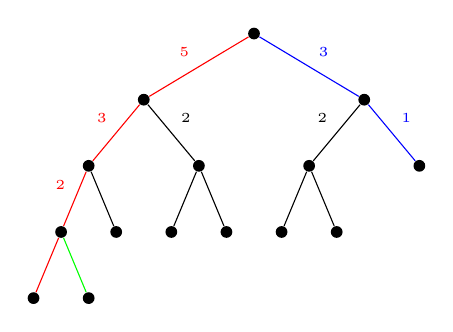
\begin{tikzpicture}[scale=0.7]

\node[circle, fill=black, inner sep=1.5pt] (root) at (0,0) {};
\node[circle, fill=black, inner sep=1.5pt] (n1) at (-2,-1.2) {};
\node[circle, fill=black, inner sep=1.5pt] (n2) at (2,-1.2) {};
\node[circle, fill=black, inner sep=1.5pt] (n3) at (-3,-2.4) {};
\node[circle, fill=black, inner sep=1.5pt] (n4) at (-1,-2.4) {};
\node[circle, fill=black, inner sep=1.5pt] (n5) at (1,-2.4) {};
\node[circle, fill=black, inner sep=1.5pt] (n6) at (3,-2.4) {};
\node[circle, fill=black, inner sep=1.5pt] (n7) at (-3.5,-3.6) {};
\node[circle, fill=black, inner sep=1.5pt] (n8) at (-2.5,-3.6) {};
\node[circle, fill=black, inner sep=1.5pt] (n9) at (-1.5,-3.6) {};
\node[circle, fill=black, inner sep=1.5pt] (n10) at (-0.5,-3.6) {};
\node[circle, fill=black, inner sep=1.5pt] (n11) at (0.5,-3.6) {};
\node[circle, fill=black, inner sep=1.5pt] (n12) at (1.5,-3.6) {};

% added nodes
\node[circle, fill=black, inner sep=1.5pt] (n13) at (-4,-4.8) {};
\node[circle, fill=black, inner sep=1.5pt] (n14) at (-3,-4.8) {};

% edges
\draw[red] (root) -- (n1) node[midway, above left] {\tiny $5$};
\draw[blue] (root) -- (n2) node[midway, above right] {\tiny $3$};
\draw[red] (n1) -- (n3) node[midway, above left] {\tiny $3$};
\draw (n1) -- (n4) node[midway, above right] {\tiny 2};
\draw (n2) -- (n5) node[midway, above left] {\tiny $2$};
\draw[blue] (n2) -- (n6) node[midway, above right] {\tiny 1};
\draw[red] (n3) -- (n7) node[midway, above left] {\tiny $2$};
\draw (n3) -- (n8);
\draw (n4) -- (n9);
\draw (n4) -- (n10);
\draw (n5) -- (n11);
\draw (n5) -- (n12);
\draw[red] (n7) -- (n13);
\draw[green] (n7) -- (n14);

\end{tikzpicture}
\end{minipage}
\hfill
\begin{minipage}{0.48\textwidth}
\centering
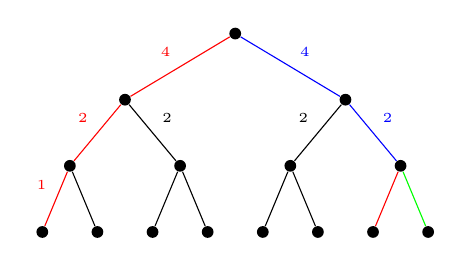
\begin{tikzpicture}[scale=0.7]

% Copy the same node layout for now; you can modify for T' later
\node[circle, fill=black, inner sep=1.5pt] (root) at (0,0) {};
\node[circle, fill=black, inner sep=1.5pt] (n1) at (-2,-1.2) {};
\node[circle, fill=black, inner sep=1.5pt] (n2) at (2,-1.2) {};
\node[circle, fill=black, inner sep=1.5pt] (n3) at (-3,-2.4) {};
\node[circle, fill=black, inner sep=1.5pt] (n4) at (-1,-2.4) {};
\node[circle, fill=black, inner sep=1.5pt] (n5) at (1,-2.4) {};
\node[circle, fill=black, inner sep=1.5pt] (n6) at (3,-2.4) {};
\node[circle, fill=black, inner sep=1.5pt] (n7) at (-3.5,-3.6) {};
\node[circle, fill=black, inner sep=1.5pt] (n8) at (-2.5,-3.6) {};
\node[circle, fill=black, inner sep=1.5pt] (n9) at (-1.5,-3.6) {};
\node[circle, fill=black, inner sep=1.5pt] (n10) at (-0.5,-3.6) {};
\node[circle, fill=black, inner sep=1.5pt] (n11) at (0.5,-3.6) {};
\node[circle, fill=black, inner sep=1.5pt] (n12) at (1.5,-3.6) {};

% reattached cherry
\node[circle, fill=black, inner sep=1.5pt] (n13) at (3.5,-3.6) {};
\node[circle, fill=black, inner sep=1.5pt] (n14) at (2.5,-3.6) {};


% edges
\draw[red] (root) -- (n1) node[midway, above left] {\tiny $4$};
\draw[blue] (root) -- (n2) node[midway, above right] {\tiny $4$};
\draw[red] (n1) -- (n3) node[midway, above left] {\tiny $2$};
\draw (n1) -- (n4) node[midway, above right] {\tiny 2};
\draw (n2) -- (n5)node[midway, above left] {\tiny 2};
\draw[blue] (n2) -- (n6) node[midway, above right] {\tiny $2$};
\draw[red] (n3) -- (n7) node[midway, above left] {\tiny $1$};
\draw (n3) -- (n8);
\draw (n4) -- (n9);
\draw (n4) -- (n10);
\draw (n5) -- (n11);
\draw (n5) -- (n12);
\draw[green] (n6) -- (n13);
\draw[red] (n6) -- (n14);

\end{tikzpicture}
\end{minipage}

\caption{Side-by-side illustration of the initial tree $T$ (left) and the tree $T'$ after balancing (right). The pruning path $\{e_i^p\}$ in red and the attachment path $\{e_i^a\}$ in blue are highlighted}
\label{fig:balancing_algorithm_trees}
\end{figure}
% endfig


Suppose that $\{\alpha_i\}_{i=1}^{2k-2}, \{\alpha_i'\}_{i=1}^{2k-2}$ are the descendant counts of $T, T'$ respectively. We claim that $\sum f(\alpha_i') \leq \sum f(\alpha_i)$, namely that this balancing operation can only decrease the overall sum. To see why, let
%
\[v = u_0 \xrightarrow{e^p_1} ... \xrightarrow{e^p_n} u_n = \ell_p, \quad v = w_0 \xrightarrow{e^a_1} ... \xrightarrow{e^a_m} w_m = \ell_a\]
%
\noindent be the paths we traverse the tree in our pruning (from $v \to \ell_p$) and grafting (from $v \to \ell_a$) operations respectively. Note that $\alpha_e = \alpha'_e$ for all edges $e \notin \{e_i^p\} \cup \{e_i^a\}$ not along either of these paths. Moreover, every edge along the pruning path loses exactly one descendant leaf and every edge along the attachment path gains exactly one leaf.  The edges in $T,T'$ are exactly the same, except for the relocation of the cherry, and hence we pair the descendant counts $\alpha_e, \alpha'_e$

\[\sum_i (f(\alpha_i) - f(\alpha'_i))=  \sum_{i=1}^{n-1} [f(\alpha_{e_i^p}) -  f(\alpha_{e_i^p} - 1)] + \sum_{i=1}^{m-1} [f(\alpha_{e_i^a}) -  f(\alpha_{e_i^a} + 1)].\]

\noindent Moreover,  by construction $m \leq n$ and $\alpha_{e_i^p} > \alpha_{e_i^a}$. This is because we always choose the larger subtree for pruning and the smaller for attaching. Thus $\alpha_{e_1^p} > \alpha_{e_1^a}$ and hence by induction
%
\[\alpha_{e_i}^p \geq \bigg\lceil \frac{\alpha_{e_{i-1}^p}}{2} \bigg \rceil > \bigg\lfloor \frac{\alpha_{e_{i-1}^a}}{2} \bigg \rfloor \geq \alpha_{e_i^a}\]
%
\noindent so $\alpha_{e_i^p} > \alpha_{e_i^a}$ is true for all $i$. Using this, we can see

\[= \sum_{i=1}^{m-1} [f(\alpha_{e_i^p}) -  f(\alpha_{e_i^p} - 1)] + [f(\alpha_{e_i^a}) -  f(\alpha_{e_i^a} + 1)] + \sum_{i=m}^{n-1} [f(\alpha_{e_i^p}) -  f(\alpha_{e_i^p} - 1)].\]

\noindent Each term in the first summand is nonnegative as $f$ is convex, and each term in the second summand is nonnegative as $f$ is increasing. Hence $\sum (f(\alpha_i) - f(\alpha_i')) \geq 0$ and the result follows.


Lastly, we argue that any tree can be converted into a balanced tree by iterating this procedure. If the subtrees of a given unbalanced vertex have size $L,R$ respectively where $L-R \geq 2$ then clearly after this procedure they have sizes $L-1, R+1$ respectively with imbalance $(L-1) - (R+1) = (L-R) - 2$. Hence the imbalance decreases by two, and if we iterate this procedure enough times we can get the imbalance to be $(L-R) \; mod(2)$, namely the vertex is balanced. Moreover, the descendant counts of any vertices not contained in one of the subtrees of $v$ are left unchanged. Hence we can start at the root and iteratively apply the procedure until the root is balanced. Then we can work our way down the tree.
\end{proof}

This type of iterative subtree balancing is reminiscent of measures of tree balance in phylogenetics, where metrics such as the Colless or Sackin indices quantify how balanced a tree is relative to the maximally balanced or maximally imbalanced (caterpillar) configurations. Tree balance statistics have long been used in phylogenetics to characterize the shapes of evolutionary trees, compare them to null models, and infer evolutionary processes such as speciation or extinction biases \cite{kersting2025_tree_balance_phylogenetic_models}.

Classical tree-balancing procedures in computer science—such as AVL trees \cite{adelson1962_avl_information_organization} and weight-balanced trees \cite{nievergelt1973_bounded_balance_binary_search_trees}—use local rotations to enforce constraints on subtree depths or sizes. Our algorithm shares the same conceptual goal of redistributing leaves to reduce imbalance, but it is purely combinatorial and does not maintain any search property.
%%%%%%%%%%%%%%%%%%%%%%%%%%%%%%%%%%%%%%%%%%
% Proof of asymptotics
%%%%%%%%%%%%%%%%%%%%%%%%%%%%%%%%%%%%%%%%%%
\section{Coalescent-Time Asymptotics}
\label{app:asymptotic-results}
\label{app:coalescent-asymptotics-proof}

\subsection{Hypoexponential Representation and Derivative Bounds}
\label{app:hypoexponential-derivative-bounds}


In this appendix, we prove Lemma~\ref{lem:asymptotics_g_k1(T)} by developing
asymptotics for the time to coalescence in Kingman's coalescent. More properties of this
coalescent time are discussed in \cite{moehle2015_absorption_time_tree_length} and
\cite{chen2013_asymptotic_coefficients_lagrange}. The paper
\cite{kersting2017_absorption_time_lambda_coalescents} further generalizes some of these
ideas to $\Lambda$-coalescents.

 We will work in slightly more generality than this chapter requires. Namely, suppose that we have positive \textbf{distinct} rates $\{\lambda_i\}_{i=1}^\infty$. Define the random variables $\{S_k\}_{k =1}^\infty$ by $S_k = \sum_{i=1}^k X_i$ for $X_i \sim \mathrm{Exp}(\lambda_i)$ independent (namely $X_i$ has density $\tau_i(x) := \lambda_i \exp(-\lambda_i x)$). Moreover, define $F_k(T) := \P(S_k \leq T)$ to be their CDFs and $f_k(T)$ their densities. If we define
%
\[C_{i,k} := \prod_{\substack{m=1 \\ m \neq i}}^k \frac{\lambda_m}{\lambda_m - \lambda_i}\]
%
\noindent then we have the following well-known explicit formulas for the CDFs and densities
%
\begin{equation}
    F_k(T) = 1-\sum_{i=1}^k C_{i,k} \exp(-\lambda_i T), \qquad f_k(T) = \sum_{i=1}^k C_{i,k} \lambda_i \exp(-\lambda_i T).
    \label{eqn:cdf_density_hypoexponential}
\end{equation}
%
\noindent See \cite{yanev2020_exponential_hypoexponential_characterizations}, for example. Moreover, we have the natural recursive relation
%
\begin{equation}
    F_k(T) = (F_{k-1} \ast \tau_k)(T) := \int_0^T F_{k-1}(x) \lambda_k \exp(-\lambda_k (T-x)) \; dx.
    \label{eqn:recursion_convolution}
\end{equation}
%
Since $S_k$ are monotonically increasing, we see $S_k \uparrow S_\infty := \sum_{i=1}^\infty X_i$ almost surely, where the limit may be infinite. To quantify the rate of convergence, define the partial sums $s_k  = \sum_{i=1}^k \lambda_i$, the remainder $R_k := \sum_{i=k+1}^\infty X_i$, and the remainder's expectation $r_k := \E R_k= \sum_{i=k+1}^\infty \lambda_i^{-1}$. We begin with explicit formulas for the derivatives of the CDF in terms of these rates $\{\lambda_i\}$.

\begin{lemma}
\label{lem:hypoexponential_derivative_properties}
    If we have positive, distinct rates $\{\lambda_i\}_{i = 1}^\infty$:

    \begin{enumerate}[label=(\roman*)]
        \item At zero, the one-sided derivatives $F_k^{(m)}(0) = 0$ for $0 \leq m \leq k-1$. The nonzero derivatives take the form
        %
        \[F_{k}^{{(k + r)}}(0) = (-1)^r \left(\prod_{i=1}^k \lambda_i\right) \left(h_r(\lambda_1,..., \lambda_k)\right),\]
        %
        \noindent where $h_r$ are the complete homogeneous symmetric polynomials
        %
        \[ h_r(\lambda_1, ..., \lambda_k) := \sum_{1\leq i_1\leq i_2 \leq ...\leq i_r\leq k} \prod_{j=1}^r \lambda_{i_j}.\]
        %
        \noindent In particular, for $r=0, 1$ we have
            \[F_k^{(k)}(0) = \prod_{i=1}^k \lambda_i, \qquad F_k^{(k+1)}(0) = -\left(\sum_{i=1}^k \lambda_i\right)\left(\prod_{i=1}^k \lambda_i\right).\]
        %
        \item The derivatives are uniformly bounded. Namely, for fixed $m$

        \[||F_k^{(m)}||_\infty \leq M_m = \max_{i=1, ...,m} |F_i^{(m)}(0)|.\]

    \end{enumerate}


\end{lemma}


\begin{proof}

% proof (i) %%%%%%%%
\noindent (i) It is easy to see that for $m \geq 1$
%
\[F_k^{(m)}(0) = (-1)^{m-1}\sum_{i=1}^k C_{i,k} \lambda_i^m\]
%
which vanishes by Lemma 2 of \cite{yanev2020_exponential_hypoexponential_characterizations} when $m \leq k-1$. To calculate the first nonzero derivatives, we will rely on the recurrence in Equation \ref{eqn:recursion_convolution}. Note that given two smooth functions $g,h : [0, \infty) \to \R$ and their convolution
%
\[g \ast h(T) := \int_0^T g(T-t) h(t) \; dt = \int_0^T g(t) h(T-t) \; dt.\]
%
\noindent Hence, by Leibniz's integral rule we have
%
\begin{equation}
    (g \ast h)'(T) = (g' \ast h)(T) + g(0)h(T) = (g \ast h')(T) + g(T)h(0).
    \label{eqn:derivatives_of_convolutions}
\end{equation}
%
\noindent By iteratively applying this to $F_k = F_{k-1} \ast \tau_k$, we see
%
\begin{equation}
F_k^{(m)}(T) = (F_{k-1}^{(m)} \ast \tau_k)(T) + \sum_{j=0}^{m-k} F_{k-1}^{(k-1+j)}(0) \tau^{(m-k-j)}_k(T),\\
\label{eqn:convolution_formula_derivatives}
\end{equation}
%
\noindent since by $(ii)$ the first $k-2$ derivatives of $F_{k-1}$ vanish. In particular, if $k > m$ we see $F_k^{(m)} = F^{(m)}_{k-1} \ast \tau_k$. Using this, we can prove $F_{k}^{(k+m)}(0)$ has the desired form by induction. Note $F_1(T) = 1-\exp(-\lambda_1 T)$ so $F_1^{(m+1)}(0) = (-1)^{m}\lambda_1 \cdot \lambda_1^m$ as desired. Moreover, $\tau_k^{(r)}(0) = (-1)^r \lambda_k^{r+1}$. Thus by induction and equation \eqref{eqn:convolution_formula_derivatives}

\[F_{k}^{(k+m)}(0) = \sum_{j=0}^m F_{k-1}^{(k-1 + j)}(0)\,\tau^{(m-j)}_{k}(0) = (-1)^m \left(\prod_{i=1}^k \lambda_i\right) \sum_{j=0}^m \lambda_{k}^{m-j} a_{k-1, j} \]
%
\noindent where $a_{k, m} := h_m(\lambda_1,..., \lambda_k)$ are our symmetric polynomials. Hence it suffices to show these polynomials satisfy the recurrence
%
\[a_{k,m} = \sum_{j=0}^m \lambda_{k}^{m-j} a_{k-1, j}.\]
%
\noindent But this is almost immediate, just by grouping terms according to the number of $i_\ell$ that equal $k$
%
\[
a_{k,m}
= \sum_{1\leq i_1\leq i_2\leq\cdots\leq i_m\leq k}
    \prod_{\ell=1}^m \lambda_{i_\ell}
= \sum_{j=0}^m \lambda_k^{m-j}
    \sum_{1\leq i_1\leq i_2\leq\cdots\leq i_j\leq k-1}
    \prod_{\ell=1}^j \lambda_{i_\ell}
= \sum_{j=0}^m \lambda_k^{m-j} a_{k-1,j},
\]
where the inner sum and product for $j=0$ are understood to equal one.
%
\noindent Hence
%
    \[F_{k}^{(k+m)}(0) = (-1)^m a_{k,m} \prod_{i=1}^k \lambda_i\]
%
\noindent takes the desired form.

% part (ii) proof %%%%%%%
\noindent (ii) Since we saw in the previous section that for $k > m$ we have $F_k^{(m)} = F_{k-1}^{(m)} \ast \tau_k$, by iteratively applying Young's convolution inequality we get
%
\[ ||F_{k}^{(m)}||_\infty \leq ||F_{k-1}^{(m)}||_\infty \cdot ||\tau_k||_1 = ||F_{k-1}^{(m)}||_\infty  \Longrightarrow  ||F_{k}^{(m)}||_\infty \leq ||F_m^{(m)}||_\infty, \quad \forall k \geq m.\]
%
\noindent Hence we can see $||F_k^{(m)}||_\infty \leq \max_{i=1,...,m} ||F_i^{(m)}||_\infty =: M_m < \infty$.

To quantify $M_m$, note that using the expression for the derivatives of $\tau_k$, we can see equation \eqref{eqn:convolution_formula_derivatives} can be re-expressed as
%
\[F_k^{(m)}(T) = F_{k-1}^{(m)} \ast \tau_k(T) + F_{k}^{(m)}(0) \exp(-\lambda_k T).\]
%
\noindent Then Young's convolution inequality implies
%
\[|F_k^{(m)}(T)| \leq ||F_{k-1}^{(m)}||_\infty \cdot (1-\exp(-\lambda_k T)) + |F_{k}^{(m)}(0)| \exp(-\lambda_k T) \leq \max \{||F_{k-1}^{(m)}||_\infty, |F_{k}^{(m)}(0)|\}.\]
%
for any $T \geq 0$. Taking the supremum over $T$ yields
%
    \[||F_k^{(m)}||_\infty \leq \max \{||F_{k-1}^{(m)}||_\infty, |F_{k}^{(m)}(0)|\}.\]
%
\noindent By induction we see $M_m = \max_{i=1,..., m}|F_i^{(m)}(0)|$ as desired.
\end{proof}



%%%%%%%%%%%%%%%%%%%%%%%%%%%%%%%%%%%%%%%%%%%%%
% CDF Asymptotics
%%%%%%%%%%%%%%%%%%%%%%%%%%%%%%%%%%%%%%%%%%%%%
\subsection{Small- and Large-Time CDF Asymptotics}
\label{app:cdf-asymptotics}
\noindent Now that we have these bounds, the main results follow. We in fact show something slightly stronger: that the relative error in the Taylor series approximation is negligible in the $T = o((s_k/k)^{-1})$ regime no matter where we truncate it.

\begin{theorem}
    If $m = \arg \min_{i=1,...,k} \lambda_i$, then the CDFs have asymptotics
        %
        \[\begin{cases}
            1-F_k(T)  \sim   C_{m,k}\exp(-\lambda_m T), & T \uparrow \infty \text{ and k fixed,}\\
            F_k(T)  \sim \frac{\prod_{i=1}^k \lambda_i}{k!} T^{k}, &  T = o((s_{k}/k)^{-1}),\\
        \end{cases}\]
        \noindent where $T = o((s_k/k)^{-1})$ denotes any sequence of pairs $(T_n, k_n)$ so that $\lim_{n \to \infty} s_{k_n}T_n/k_n = 0$. More generally, in the same $T = o((s_k/k)^{-1})$ regime and for any finite $m \geq 0$
        \[\frac{F_k(T) - \sum_{r=0}^{m} a_{r,k}}{a_{m, k}} \to 0, \qquad a_{r,k} := (-1)^r \frac{h_{r}(\lambda_1,..., \lambda_k)\prod_{i=1}^k \lambda_i }{(k+r)!} T^{k+r}.\]
\end{theorem}


% proof of thm %%%%%%
\begin{proof}
 For $k$ fixed, the exponential in equation \ref{eqn:cdf_density_hypoexponential} with the smallest rate decays the slowest, so $1-F_k(T) \sim C_{m,k}\exp(-\lambda_m T)$ as $T \to \infty$. For the other asymptotics, first fix $k$ and let $h_{r,k} := h_r(\lambda_1, ..., \lambda_k)$ be our symmetric polynomials and $p_k = \prod_{i=1}^k \lambda_i$. Since $F_k(T)$ is the sum of a finite number of exponentials, its Taylor series at zero converges to $F_k(T)$ for all $T$. Moreover, (i) of Lemma \ref{lem:hypoexponential_derivative_properties} above tells us $F_k^{(k+r)}(0) = (-1)^r p_k h_{r,k}$. Thus, let
%
\[a_{r,k} = (-1)^r \frac{p_k h_{r,k}}{(k+r)!} T^{k+r}\]
%
\noindent denote the $(r+1)^{th}$ nonzero term in the Taylor series expansion about zero. Suppose that we approximate $F_k(T)$ by the first $(m+1)$ nonzero terms of its Taylor series about zero. We can measure the approximation error relative to the last term $a_{m,k}$ to see
%
\[\frac{F_k(T) - \sum_{r=0}^{m} a_{r,k}}{a_{m, k}} = \sum_{r=1}^\infty (-1)^r\frac{h_{m+r}/h_mT^r}{(k+m+r)_r}\]

\noindent where $(x)_r = x(x-1) \cdot ... \cdot (x-r+1)$ denotes the falling factorial. We will now bound the right hand side by a geometric series.

Note that trivially $h_{r+1} \leq h_r s_k$ as the former includes all monomials of degree $(r+1)$ in $\{\lambda_i\}_{i=1}^k$ with coefficient one, and the latter has all the monomials with coefficient at least one. Hence $h_{m+r} / h_m = \prod_{i=0}^{r-1} h_{m+i+1}/h_{m+i} \leq s_k^r$. Using this and the simple bound $(k + m + r)_r \geq k^r$ we get

\[\bigg|\sum_{r=1}^\infty (-1)^r\frac{h_{m+r}/h_mT^r}{(k+m+r)_r}\bigg| \leq \sum_{r=1}^\infty \left(\frac{s_kT}{k}\right)^r = \frac{s_kT/k}{1 - s_k T/k}\]

\noindent for $|s_kT/k| < 1$. When $T = o((s_k/k)^{-1})$, this tends to zero.  Thus in this regime
%
\[\frac{F_k(T) - \sum_{r=0}^{m} a_{r,k}}{a_{m, k}} \to 0,\]
%
 \noindent as desired. In particular
%
\[F_k(T) = (1 + o(1)) \frac{\prod_{i=1}^k \lambda_i}{k!} T^{k}.\]
%
\end{proof}

%%%%%%%%%%%%%%%%%%%%%%%%%%%%%%%%%%%%%%%%%%%%%
% Gap Asymptotics
%%%%%%%%%%%%%%%%%%%%%%%%%%%%%%%%%%%%%%%%%%%%%
\subsection{Gap Asymptotics}
\label{app:gap-asymptotics}

\noindent The following statement gives us a sense of how fast our coalescent probabilities $g_{k,1}(T)$ will saturate as $k \to \infty$.

\begin{theorem}[Gap Asymptotics] If $\sum_{i=1}^\infty \lambda_i^{-1} < \infty$, then $F_k \to F_\infty$ uniformly. Quantitatively, the gap $\Delta_k(T) = F_{k}(T) - F_\infty(T)$ has asymptotics
        \[\Delta_k = (f_\infty + o(1))r_k.\]
\end{theorem}

  \begin{proof}
          Dini's theorem already guarantees that $F_k \to F_\infty$ uniformly. Here, we will get quantitative control on the rate of convergence. Note that (ii) of Lemma \ref{lem:hypoexponential_derivative_properties} implies the functions $f_k$ are uniformly bounded by $M_1$ and uniformly $M_2$-Lipschitz. Thus they form a uniformly equicontinuous family which is uniformly bounded.  Since $S_k \Rightarrow S_\infty$, as a consequence of \cite{boos1985_converse_scheffe} converse to Scheffe's lemma, we see $f_{k} \to f_{\infty}$ uniformly on $[0, \infty)$. Now, note that by conditioning on the tail $R_k$, as $S_k \indep R_k$
        %
        \[\P(S_\infty \leq T) = \int_0^\infty \P(S_k \leq T-r) \P(R_k \in dr) = \E F_k(T-R_k).\]
        %
        \noindent Hence by Taylor expanding the CDF $F_{k}$ we get
        %
        \[\Delta = \E_{ R_k} [F_{k}(T) - F_{k}(T-R_k)] = f_{k}(T) \cdot \E R_k + \frac{1}{2}\E \left(f'_{k}(\xi(R_k)) R_k^2\right),\]
        %
        \noindent where $\xi(r) \in (T-r, T)$ for every $r$. Note that $\mathrm{Var}(R_k) = \sum_{i=k+1}^\infty\lambda_i^{-2}\leq r_k^2$, implying $\E R_k^2 \leq 2r_k^2$. Since $||f'_{k}||_\infty \leq M_2$ is uniformly bounded by (iii) and as $f_{k}(T) \to f_{\infty}(T)$ uniformly as $k \to \infty$
        %
        \[\Delta_k(T) = f_\infty(T) r_k + (f_k(T) - f_\infty(T))r_k + O(r_k^2) = f_\infty(T) r_k + o(r_k).\]
        %
        \noindent More specifically, since $M_2 = \max \{|F_1''(0)|, |F_2''(0)|\} =  \lambda_1\max(\lambda_1, \lambda_2)$
        \[||\Delta_k(T) - f_\infty r_k||_\infty \leq ||f_k - f_\infty||_\infty r_k + \lambda_1\max(\lambda_1, \lambda_2) r_k^2 = o(r_k)\]
        \noindent so the rate of convergence is uniform in $T$.
  \end{proof}


  Lemma \ref{lem:asymptotics_g_k1(T)} then just follows from the special case of Kingman's coalescent, where we have rates $\tilde{\lambda}_i = \binom{i+1}{2}$. Note the indexing is slightly different here than in the main paper: it is shifted down by one, but otherwise the same. Here we have
%
\[r_k = \sum_{i=k+1}^\infty \frac{1}{\binom{i +1}{2}} = \frac{2}{k+1}, \qquad s_k = \sum_{i=1}^k \binom{i + 1}{2} =  \frac{k(k+1)(k+2)}{6} = \Theta(k^3).\]
%
\noindent Moreover, a simple induction shows that $C_{1,k} = 3k/(k+2)$. Hence we get asymptotics

    \[F_k(T) \sim \begin{cases}
        1-\frac{3k}{k+2}\exp(-T), & T \uparrow \infty  \text{ and k fixed,}\\
        \frac{(k+1)!}{2^k} T^{k}, &  T = o(k^{-2}).\\
    \end{cases} \qquad \Delta_k(T) = (f_\infty(T) + o(1)) \cdot \frac{2}{k+1}\]
\end{subappendices}
